\UseRawInputEncoding
\documentclass[12pt, a4paper, oneside]{book}

\usepackage{helvet}
\usepackage{hyperref}
\usepackage{graphics}
\usepackage{graphicx}
\usepackage{listings}
\usepackage{textcomp}
\usepackage[
	a4paper,
	outer=2cm,
	inner=4cm,
	top=2cm,
	bottom=2cm
]{geometry}
\usepackage{float}
\usepackage{tabularx}
\usepackage{xcolor}
%\usepackage[disable]{todonotes}
%\usepackage{color, soul}
\usepackage{amsmath}
%\usepackage{algorithmicx}
%\usepackage[noend]{algpseudocode}
%\usepackage{algorithm}
\usepackage{framed}
\usepackage{subcaption}
%\usepackage{titlepic}
%\usepackage{fancyhdr}
%\usepackage[simplified]{styles/pgf-umlcd}
\usepackage{shorttoc}
\usepackage{url}
%\usepackage{paralist}
\usepackage{dirtytalk}
%\usepackage{verbatim}

\definecolor{grey}{rgb}{0.9, 0.9, 0.9}
\definecolor{dkgreen}{rgb}{0,0.6,0}
\definecolor{dkred}{rgb}{0.6,0,0.0}

\lstdefinestyle{DOS}
{
    backgroundcolor=\color{black},
    basicstyle=\scriptsize\color{white}\ttfamily,
    stringstyle=\color{white},
    keywords={}
}

\lstdefinestyle{makefile}
{
    numberblanklines=false,
    language=make,
    tabsize=4,
    keywordstyle=\color{red},
    identifierstyle= %plain identifiers for make
}

\lstset{
  language=Python,                % the language of the code
  escapeinside={\%*}{*)},
  basicstyle=\footnotesize\ttfamily,
  numbers=left,                   % where to put the line-numbers
  stepnumber=1,                   % the step between two line-numbers. If it's 1, each line
  numbersep=5pt,                  % how far the line-numbers are from the code
  backgroundcolor=\color{white},      % choose the background color. You must add \usepackage{color}
  showspaces=false,               % show spaces adding particular underscores
  showstringspaces=false,         % underline spaces within strings
  showtabs=false,                 % show tabs within strings adding particular underscores
  frame=single,                   % adds a frame around the code
  rulecolor=\color{black},        % if not set, the frame-color may be changed on line-breaks within not-black text (e.g. comments (green here))
  tabsize=2,                      % sets default tabsize to 2 spaces
  captionpos=b,                   % sets the caption-position to bottom
  breaklines=true,                % sets automatic line breaking
  breakatwhitespace=false,        % sets if automatic breaks should only happen at whitespace
  keywordstyle=\color{blue},          % keyword style
  commentstyle=\color{dkgreen},       % comment style
  stringstyle=\color{dkred},         % string literal style
  columns=fixed,
  extendedchars=true,
  frame=single,
}

%\renewcommand{\chaptername}{Topic}

% New definitions
%\algnewcommand\algorithmicswitch{\textbf{switch}}
%\algnewcommand\algorithmiccase{\textbf{case}}
%\algnewcommand\algorithmicassert{\texttt{assert}}
%\algnewcommand\Assert[1]{\State \algorithmicassert(#1)}%
% New "environments"
%\algdef{SE}[SWITCH]{Switch}{EndSwitch}[1]{\algorithmicswitch\ #1\ \algorithmicdo}{\algorithmicend\ \algorithmicswitch}%
%\algdef{SE}[CASE]{Case}{EndCase}[1]{\algorithmiccase\ #1}{\algorithmicend\ \algorithmiccase}%
%\algtext*{EndSwitch}%
%\algtext*{EndCase}%

%\pagestyle{fancy}
%\fancyhf{}
%\fancyhead[RO, LE]{\small \rightmark}
%\fancyfoot[RO, LE]{\small \thepage}

\newcommand{\blank}[1]{\hspace*{#1}}

\begin{document}

\frontmatter

\begin{titlepage}
\vspace*{5cm}
\begin{center}

\includegraphics[width=.5\textwidth]{figures/EdNapUniLogoCMYK}~\\[1cm]

\textsc{\Large Web Technologies}\\[1.5cm]

\textsc{\LARGE \bfseries SET08101/401/801 }\\[0.5cm]

\hrulefill \\[0.4cm]
{\huge \bfseries Notes \& Workbook 2020-2021 \\[0.4cm] }
\hrulefill \\[1.5cm]

\begin{minipage}{0.4\textwidth}
\begin{flushleft} \large
\textbf{Dr Simon Wells} \\
\end{flushleft}
\end{minipage}

\vfill

\end{center}
\end{titlepage}

%\shorttoc{Overview}{0}

\setcounter{tocdepth}{2}
\cleardoublepage
\tableofcontents
%\listoffigures
%\listofalgorithms
\addtocontents{toc}{~\hfill\textbf{Page}\par}

\mainmatter


%%%%%%%%%%%%%
%%%%%%%%%%%%%
%%%%%%%%%%%%%       ADMIN
%%%%%%%%%%%%%
%%%%%%%%%%%%%



\chapter{Administrivia}

\section{Introduction}
\label{intro}

\paragraph{} Welcome to the Web Technologies module from Edinburgh Napier University. This module has a slightly different structure to many modules so it's worth reading through this guidance before you get stuck into the good stuff.

%\paragraph{} This module is about the Web, what the Web is, what we can currently do with the Web, and what the Web might be like in the future. Rather than focus on the user side of web technology, such as CSS and Javascript, which we've all probably seen in other modules (particularly \emph{web tech}, the pre-requisite for this module), we are going to take a more holistic approach and examine both the server and the client side. We shall look at HTTP (the core of all web technologies) and learn how APIs, Web Services, \& RESTful architectures are built to move data around. We will then delve into some more topical discussions, starting with security \& privacy on the web, then looking at adding intelligence (Semantic Web), adding increased, scalable interaction (Realtime Web) and private, anonymous, and un-censorable web-technologies (Dark Web). We wrap up the module by examining a few technologies that might form the basis of future web capabilities like Blockchain and IPFS. Throughout the module you should be using the topics as a starting point. A starting point for your own, self-directed, exploration of the topic in more depth. Because we can only really survey any given aspect during contact time; the real knowledge comes from you digging into it in depth. Also a starting point for you to critically reflect on your own experiences and responses to the topics and issues that we raise in class. Whilst the Web itself is a technical mechanism, a tool for moving data around, it also operates in a very complex socio-technical context that currently affects, and will likely affect to an even larger degree in the future, all our lives.

%\paragraph{} Lectures and labs will not necessarily align neatly, the labs will progress, on a week-by-week and chapter-by-chapter basis to form a first course in ``\emph{developing server side web-apps using Python and associated professional practises in a Linux-based environment}''. The lectures will summarise some of this material, providing an opportunity to talk over what we learned in the lab, but primarily, the lectures are an opportunity for us to discuss many other aspects of the Web, focussing in particular on two aspects. Firstly, the structure of the existing Web. Secondly the various facets of Web technologies that influence or alter the way that we use, manipulate, navigate, and share information. These break down into a series of named facets: the semantic web, the realtime web, the dark web, and the permanent web, each of which imposes its own constraints on and proffers opportunities for what the Web is and can do. By looking at each of these in turn we should gain some insight into how the Web is developing, the directions it might take in the future, and perhaps, suggest areas that we can usefully and positively affect.

\paragraph{} How should we use this workbook? Ideally we would work through it on a chapter-by-chapter basis supplementing our work with background reading and wider exploration of each topic introducted. Some chapters will take longer to complete than others, and other chapters will need to be returned to multiple times. This is particularly true for the first two chapters. To learn both Linux and Python in a fortnight is a tall order so I'd suggest working iteratively, do enough to make some progress, then frequently return to the respective chapters to learn a little more, usually by following the links and footnotes to further practise materials.

\paragraph{} In the first week work through the first chapter in the lab section of the workbook. You can read ahead if you want but don't try to run any Flask web-apps on the dev server until you've been assigned your personal virtual server to run your own web-apps on. This week is mostly concerned with the foundation of our learning environment. Logging in, learning to navigate and do simple tasks at the command line, using a non-gui text editor, and using Git. There are links, usually in footnotes, throughout the chapter, for example, to practise the Linux command line then there are online web sites like the \emph{LinuxZoo}\footnote{\url{http://www.linuxzoo.net}} that you can use to practise your skills. Similarly, the links to Vim practise tutorials, particularly the Vim game, will help you practise the skills you need to work efficiently in subsequent weeks. Finally, make sure to work through the linked Git tutorials and ensure that you are confident that you understand each of these tools and their place within the learning environment before moving on to subsequent chapters. 

\paragraph{} Each chapter is meant to cover about an entire week of study, so don't rush through things within the scheduled lab session just to tell yourself the you've done all the work. As I mentioned in the introduction, topics, whether in lectures or labs are meant to be a starting place, a framework to guide your self-directed study, but not the totality of your learning. 

\paragraph{} In subsequent weeks you will start to build knowledge of the Python language and the Flask library which provides functionality for building server-hosted web-apps. The next chapter, on Python, is meant to cover at least a weeks work and deliberate practise. Mostly that week is concerned with developing basic skills in a new language, Python, which is actually quite a challenge. This is not because Python is particularly difficult but because learning a computer language well takes time and effort and you have to start somewhere. Subsequent weeks will require you to work through various chapters of the workbook. You will find that as you progress you will want to skip ahead to different sections, especially once the assessments are released and you want to include specific functionality in your coursework. So after about chapter 3 I expect that many of you will navigate your own path through the remainder of the workbook. The only proviso is that you should aim to have worked through every chapter by the end of the module.


\section{Reading This Book}
\label{readme}
\paragraph{} 

\begin{figure}[H]
\centering
\includegraphics[width=0.8\textwidth]{figures/reading-order.pdf}
\label{fig:reading-order}
\end{figure}






%%%%%%%%%%%%%
%%%%%%%%%%%%%
%%%%%%%%%%%%%       NOTES
%%%%%%%%%%%%%
%%%%%%%%%%%%%




%\part{Notes}



%%%%%%%%%%%%%
%%%%%%%%%%%%%
%%%%%%%%%%%%%       CHAPTER 1
%%%%%%%%%%%%%
%%%%%%%%%%%%%


\chapter{The World Wide Web}
\label{www}
\paragraph{} In this unit we begin the module with an introduction to the Web and an overview of the technologies which it comprises. From this starting point we can use subsequent units to take deeper dives into the various specific tools and technologies so that we can build a balanced and professional toolbox of Web related skills. You've probably used the web before, even if only to access this module, but more likely it is a part of your daily life so you probably have a number of preconceived ideas about how it works, how it should work, and where it is annoying and in need of improvement. You might also have had some previous experience in the Web. This is good but not necessary. We'll start from scratch in our approach to the Web which is an opportunity to reconfirm your ideas if you already know some parts and an opportunity to build new skills and understanding otherwise. 
%Practical activities for this unit are in the linked pdf file (unit1_activities.pdf). You should balance your time between working through the reading and reflective exercises in this unit on Moodle, and working through the linked activities separately in order to develop your practical skills.
 
\paragraph{} Before we can go anywhere, we should really know how we got here. This is important because the Web has been developed incrementally over around 30 years. However it is also based upon ideas that go back to at least 1945 when Vannevar Bush described the ideas of Hypertext and an associated machine, the Memex, and probably earlier. The Web, on the most basic level is really a conceptual tool for making knowledge capture, communication, and reasoning easier, but over the years there has been feature creep to do an awful lot more.
We are going to spend a little time in this unit doing a potted history of the Internet, the Web, Hypertext, DOM, \& Basic Web Architecture (Servers \& Clients). We'll then build upon, and iterate over this, iteratively deepening our knowledge and skills in subsequent units.
Whilst you are reading and thinking, consider the following question, What happened technologically \& socially, that lead to the situation we are in now and gave us the Web that we have now? 
By thinking about these things, and considering the tools that underpin the Web, we begin to construct a framework for understanding how it all fits together so that we can better use and develop our skills later.
 
vThis specific unit covers a lot of ground and it can be difficult to see how it all fits together at first. We will cover the following topics: Communication, The Internet, Internet Protocols, HTTP, Hypertext, the invention of the Web, HTML, Servers, Web-clients, Browsers, Basic Web Architecture, the client-server model, and the DOM. All are important topics when considering the Web, especially the process of getting a web page from a given Internet server to your web browser There is no single route through all of these topics as, like the web itself, they form a network of interconnected topics which each play their part in that story of getting a file from a remote server and turning it into a page in your browser. Let's consider a few scenarios:
For example, there is a historical story involving how people have thought about communicating ideas. Most ideas are hierarchically organised and related to other ideas, which lead to concepts for arranging ideas as "hypertext".

\paragraph{} There is also a computer communication story. For a computer to be able to move (communicate) information from one place to another it requires a network of multiple computers (the Internet) and agreements on how the communication should occur. These agreements are known as protocols. The Web relies on a hierarchy of protocols for things like finding another computer (using addresses call Internet Protocol, or IP, addresses), then transporting messages between the computers once they can find each other (using the Transmission Control Protocol ,or TCP), then because there are lots of different kinds of messages that computers can understand, they need a protocol for communicating web pages instead of other messages such as email data, or instant messages. This is achieved using the HyperText Transport Protocol (HTTP) which is responsible for moving Web data around. But Web data can comprise lots of different things, including the page itself (using HTML), the way the page should be presented (defined using CSS), and any dynamic functionality that the page should have (using JS).
There is also an organisational story. Whilst every computer on the Internet has an IP address (is a part of the Internet) not all of them are parts of the Web. Also, different machines play different roles, i.e. in requesting a page, serving a page, and displaying a page. So a server will provide pages to clients who make requests, and requests are made by software called "user agents" the most common type of which is the users browser. The browser and server are organised in terms of a client server organisational model.
As you go through the remaining parts of this unit, it can be worth returning to this overview to try to understand how the various parts relate to each other.


\paragraph{} So let's start by considering communication. The primary thing that the Web does is to communicate information from one place to another. For a computer to be able to communicate this information usefully, that is so that the computers at each end of the communication can understand what to do with the information, there needs to be an agreement on how the communication should proceed and how the  contents of the communication should be structured and understood. This shouldn't surprise you. Think about how you communicate with other people. For most of us, the primary means is through language. Amongst other things, successful communication between people using language involves a shared language, and some common vocabulary and understanding of the domain that the people are communicating about. The advantage that people have is that they have a brain which can solve problems and gloss over the gaps in understanding. Computers don't have this advantage, they need every aspect to be precisely specified in an unambiguous fashion.

\paragraph{} The solution, for computers is to use protocols to underpin communication. Protocols are agreements for how to communicate and they closely specify, for everything within the scope of a communication, exactly what is legal, and what is not. This means essentially that a protocol defines what a message, from one speaker to another can consist of. Any message that doesn't fit what the protocol defines is considered wrong and there are various ways to handle such wrong, garbled, incomplete, etc. messages. Computer protocols are agreements that are specified with sufficient clarity and lack of ambiguity that a computer can follow them automatically.

\paragraph{} The Internet and the Web are really just communication methods (protocols) - agreements for how two machines can exchange information. The Web itself is just one specific way that machines can exchange information. Let's now explore a couple of these concepts in some more detail...

\section{The Internet}

\paragraph{} The Internet is a global system of interconnected computer networks. Over the years there have been many different protocols underpinning computer networks, because what else is a network but a way to move information, or communicate information, between different machines. Over the years some of these protocols have become standard, and others have become obsolete. The modern Internet is currently built on a limited number of shared \& agreed protocols. These are the Internet Protocol suite which comprises the Transmission Control Protocol (TCP) and the Internet Protocol (IP). Together these are often referred to as "TCP/IP". 

\paragraph{} IP is used to govern how machines on the Internet find each other. To do this they use IP addresses, essentially numbers that are formatted as dotted-quad layouts like this:\\
	134.16.46.98
\paragraph{} Occasionally you might see IP addresses in your browsers address bar. Every Web site is stored on and "served" by web server software. This software runs on a hardware server which is not only a part of the web but is also a part of the Internet, i.e. every web site is a part of the Internet. Every web host is a part of the Internet. However, not every Internet host is a part of the web. The Internet is much bigger and incorporates functionality that is not part of the web. 
\paragraph{} Every Internet host has an IP address which is used to find other machines. The exact mechanism for finding machines from their IP address, which is literally about identifying a specific piece of hardware somewhere in the world, is outside the scope of this module, but the correct functioning of IP is essential to the working of the web. Think of an IP address as being analogous to, but not exactly the same as a postal address or a phone number, or a GPS location, a way to identify one entity, to distinguish it from others, and to locate it.
\paragraph{} TCP works with but is different to IP. Once you've located a machine, via its IP address, TCP is used to communicate data between that machine and any other machine that has an IP address. TCP is the basic mechanism for transmitting data between Internet hosts and controlling that process. Importantly, if something goes wrong during transmission, TCP has lots of mechanisms for repairing the communication. It is designed to be reliable so that a piece of software can send information, i.e. a message, to another host with guarantees that the communication will either fail or succeed. The sender and receiver don't have to worry about how the data actually gets from one to the other.
\paragraph{} An important concept here is that each protocol has its own responsibilities and they are designed to work both independently but complementary to each other. We can't send a message without knowing where it's going, but just knowing the destination doesn't necessarily tell us how to get the message to that destination. We should also consider that these protocols not only work independently but still in a complementary fashion, but also that they are designed to be layered. That is the current Web assumes that there are lower level protocols which are responsible for finding other Internet hosts, moving data to them, and returning the results. TCP/IP don't need to be the lower level protocols, and others exist, but they are the default that the modern Internet and Web currently use.
\paragraph{} The development of TCIP/IP and other networking protocols specific to the Internet dates back to research in the 1960’s which was commissioned by the US government. The aim was to build robust, fault tolerant communication via computer networks. To a large degree this has succeeded. The World Wide Web (or just Web) is just one information resource/service that communicates using the Internet (although people often use the terms interchangeably).


\section{Internet Protocols}
\paragraph{} In the last section we discussed how the Internet and the Web are built on the idea of layers of protocols. Formally there is a seven layer model called the OSI model that defines all of these layers and their various responsibilities. We don't need to know about all of them for this module so will concentrate on just those necessary to understand how the Web fits into the idea of the Internet and networks.
\paragraph{} Let's explore this a little further. On the lowest level that we'll consider here is the link layer, think of this as both the physical infrastructure, such as your WiFi or ethernet cable. It is concerned mostly with reliably moving information from place to place. Although this seems similar to TCP above, it is much lower level and the main difference is that the link layer doesn't care about how that information is broken up into packets or reassembled, it only cares that the stream of data it is given is reproduced at the other end. In comparison, TCP takes a particular approach to breaking up the data to transmit into packets, and uses specific algorithms to reassemble those packets into a whole at the other end, and also to identify and retransmit lost or broken packets. A similar protocol that works at the same level as TCP is the User Datagram Protocol (UDP) which doesn't provide the same guarantees on message integrity that TCP does. However the trade-off here is that UDP can be more efficient and faster to communicate information, with all of the risks associated with a send and forget communication protocol. We have these different protocols to enable us to use computer networks to communicate different information in different ways. Perhaps consider it as analogous to the difference between the different ways of physically sending messages around the world. We could write a postcard, or a letter in an envelope, a package or box, right up to a shipping container (and possibly other mechanisms as well but these are fairly standard).
\paragraph{} As we talked about before, once we have two networked machines (link layer) that can transmit data, they need a mechanism that enables them to address messages to specific machines, which is the role of the Internet layer and IP. Once we have a machine that we can identify individually we can use the transport layer (TCP) to move data in a specific way to the destination. It is only at this point, once we have the link, internet, and transport layers that we look at the application layer. It is this layer at which the Web protocols operate. The HyperText Transport Protocol (HTTP) is one example of this that we will investigate next but there are lots of other applications layer protocols which govern other tasks like email (the IMAP and POP protocols) or turning domain names (web addresses) into IP addresses so that, given a web address or URL (different names for the same thing) we can tell the IP protocol which machine we want to communicate with. Although people generally think of websites in terms of domain names, our computers only care about IP addresses when it comes to finding a given web server.
\paragraph{} To summarise, we have:
\begin{itemize}
\item Link Layer: Ethernet/Wifi
\item Internet Layer: IP
\item Transport Layer: TCP
\item Application Layer: DNS, HTTP, IMAP, POP 
\end{itemize}


\section{The HyperText Transfer Protocol (HTTP)}
\paragraph{} Just a little more on protocols before we consider some other aspects of the Web. The HyperText Transfer Protocol (HTTP) is our application layer protocol that is critical to facilitating the Web. Other protocols like TCP and IP don't care that the data they are transmitting or the machines between which they are moving the data are Web machines or not. Those protocols can transmit lots of data for different reasons and many of those reasons are not related to the Web.  When information arrives at a machine and is routed to software that understands HTTP it is treated as Web data. HTTP is concerned primarily with moving hypertext between Internet hosts. We'll consider what we mean by hypertext in the next section but for the moment we can think of it as being text documents. Although the modern web can manage to handle much more than just text the default is still for HyperText Markup Language (HTML) documents. HTTP is concerned with moving these documents around, requesting particular documents and processing the responses, and delegating the actual movement of the document to lower level protocols along the way. Note that HTTP does much more than just merely governing requesting documents and responding with the correct document. It also has the mechanism for responding in different ways depending upon the request made, or how successful the request was. It is this additional functionality that enables rich, server generated behaviour and on the fly page creation, but these aspects of HTTP are outside the scope of this module, although you are encouraged to do some additional background reading if it interests you. A good place to start is with the W3C specification if you want the gory details: \\
	\url{https://www.w3.org/Protocols/}
\paragraph{} HTTP is an application layer protocol for distributed and collaborative hypermedia/hypertext systems. It is based upon a request-response protocol that uses the client-server model. We'll investigate the client-server model in a little while but the basic idea is that the Client (i.e. your Web browser) makes a request. This is probably due to the user making a choice such as clicking on a link or typing in a web address. This request gets passed down the layers of the networking stack, transmitted to the remote machine, and heads back up the networking stack until it reaches the server software that understands HTTP.  Mostly though we can ignore the full stack and just consider that there is an HTTP server (software running on an Internet connected computer) that listens for requests and responds according to what the protocol allows. Any other response is problematic and will cause some form of error or failure in the communication.

\paragraph{} The HTTP Server stores resources and returns a response that may include providing access to those resources. For our purposes in this module those resources should be considered to be the things that you'd commonly expect a web site to provide, e.g. HTML pages, associated files in the CSS and JS languages that the HTML pages reference, and any other media like images, videos, or audio that the pages want to make use of.
\paragraph{} These request-response cycles occur as part of an HTTP Session. This is a sequence of request-response transactions transmitted over TCP.  One thing to note at this point is that Internet hosts can listen on different ports. The default port for the Web is port 80. In fact it is so common that most browsers don't display that the address it is connecting to is listening on port 80. A web client can connects to any legal port on any legal IP address. HTTP servers listen on that port. Whilst the default is 80 you might occasionally see other ports in your address bar, for example 8080 which is also reasonably common but some development servers run on other ports like 5000. If you see other ports, don't worry.

\paragraph{} HTTP requests are more than just a simple request to retrieve a web page, They can also involve lots of other request Methods. These methods are usually referred to as  HTTP verbs, e.g. GET, HEAD, POST, PUT, DELETE, OPTIONS, and PATCH to name a few. These verbs are essentially actions that the request is asking to be performed. The most common is HTTP GET. This is asking to retrieve or "GET" the resource (web page or HTML document) that is being asked for and return it to the client. A client makes a request and the requested resources is transmitted back to the client. What is transmitted between the client and server though is just plain text. HTML web pages are plain text, CSS files are plain text, and javascript files are plain text. They are readable and understandable by people. If you were to eavesdrop on the connection between client and server you would see text passing by containing the HTML, CSS, or JS content of the files that are being requested and then "served" up. Note that modern versions of HTTP will retrieve binary files, e.g. for audio and video, but the default is for plain text, a simple and robust encoding mechanism that is easily inspectable without specialised tools. It is this focus on plain text file, the same kind of files that any text editor can produce, which is arguably a part of making the Web so successful. Anyone with a text editor can produce the files that will make up a web page. If they then put those pages on a web server, then voila, you have published a web site.
\paragraph{} Before we finish up this introduction to HTTP, note that by default HTTP is insecure. The transmission of information is in plain text and any one machine between source and destination could intercept or manipulate it. This risk has largely been mitigated by the use of secure variants of HTTP, such as HyperText Transfer Protocol Secure (HTTPS) \& HTTP Strict Transport Security (HSTS). Browsers are slowly moving towards defaulting to HTTPS addresses. The main difference between HTTPS and HSTS is that HSTS is more strict about how it deals with mixture of secure and insecure resources on a single page. HSTS mandates for a given page that all resources on that page are served securely. This is an example of the slow improvement of Web and Internet protocols.


\section{Hypertext}
\paragraph{} In the last section we discussed HTTP, a protocol for transferring hypertext resources between Internet hosts, but we didn't really define what we meant by hypertext. So let's square that away right now. Hypertext is a term that was coined byTed Nelson as part of the Xanadu research project sometime around 1965. This was as part of a model for linked content, the idea that a concept is related to other concepts and that it would be useful to create links between concepts within and between documents so that instead of reading a page, and then reading another page in linear fashion, as we traditionally read books, instead it is useful instead to be able to follow the thread of related ideas wherever they may take us. The following diagram illustrates this idea schematically, starting with the home page highlighted in orange, individual sections of text are linked to other pages which, in turn contains links to other pages, and so on.

\begin{figure}[H]
\centering
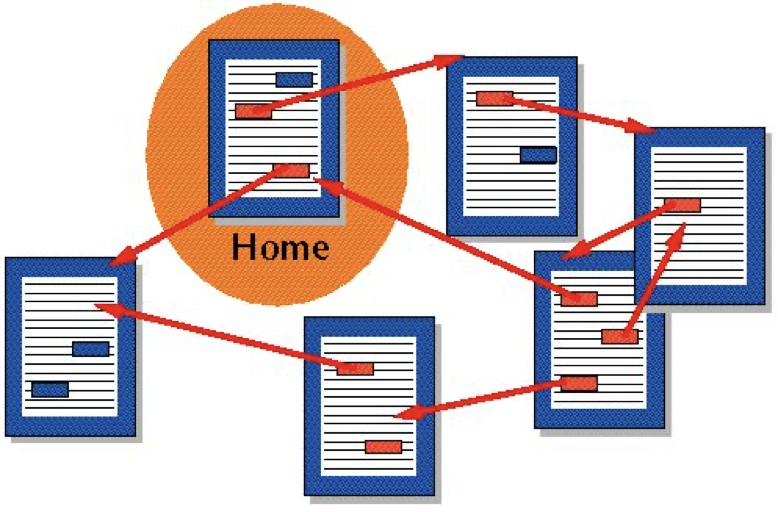
\includegraphics[width=0.4\textwidth]{figures/hypertext.png}
\label{fig:hypertext}
\end{figure}


\paragraph{} Ted Nelson didn't invent this idea though, an earlier incarnation which was visionary but came before the technology was capable was in an article by Vannevar Bush in 1945. Bush proposed the Memex, an attempt to turn this idea for turning information into a searchable and interlinked database of knowledge, however he was limited by the capabilities of 1940's technology. It is well worth reading Bush's article which can be found here:
	\url{https://www.theatlantic.com/magazine/archive/1945/07/as-we-may-think/303881/}

\paragraph{} But it is arguable that Bush didn't really invent this concept either. Before the Memex proposal we already had books that work in a similar, albeit manual and non-computational way. Dictionaries, Thesauri, and Encyclopedias also work in a similar way, referencing other sections and entries within themselves, other volumes in the collection, and other books. Encyclopedias in particular are interesting to consider because they often have summary books and indexes that give different ways to approach the articles contained within the encyclopedia proper.
\paragraph{} A modern incarnation of hypertext that is quite well defined and circumscribed is Wikipedia. Consider how you start on one Wikipedia page and then follow links to other pages until you've lost an entire afternoon discovering things you never thought that you'd want to know. This is hypertext. Text is displayed on an electronic device that incorporates references, called Hyperlinks, to other text. These Hyperlinks can be followed or navigated immediately. By doing this, text becomes non-linear as a result - instead of one page following the next we can jump between them, consuming them in whichever order makes most sense. 
\paragraph{} Note that the modern web goes beyond just links between text and other forms of media are often consumed on the Web now so you will often find the related term hypermedia used. The terms hypertext and hypermedia are frequently used interchangeably.
\paragraph{} One implementation of the hypertext idea is in HTML.  Whilst the bulk of HTML is about describing or "marking up" text documents one part of HTML concerns defining links within and between documents. Even just getting this far into the module, you'll already have navigated a whole bunch of hyperlinks as you've "browsed the web". Browsing the web is just another phrase for following hyperlinks or using hypermedia. 
\paragraph{} So the Web itself is an implementation of a hypertext system as well. That said it isn't the only possible implementation of a hypertext system, it's just the most prevalent one that we have now. Perhaps we should now consider how we ended up with the particular implementation of a hypertext system that we call "the Web"?


\section{Invention of the Web}
\paragraph{} The Web, or more formally, the World Wide Web (WWW) is an implementation of a hypermedia system. It was invented in 1989 by Sir Tim Berners-Lee whilst he was working at CERN. This involved developing HTTP to move documents around and HTML to structure and define documents themselves, with embedded links between them. The first web browser was written in 1990 but it was 1992 before there was really a usable and publicly accessible web browser (but which was very different to what we have now).

\begin{figure}[H]
\centering
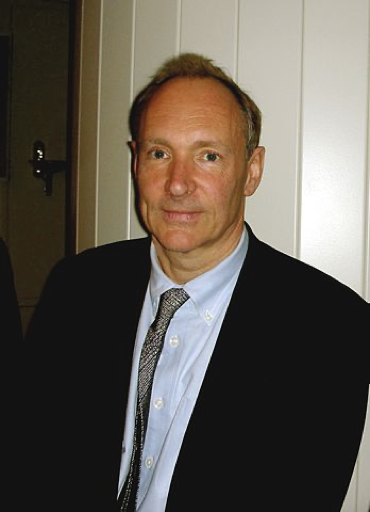
\includegraphics[width=0.8\textwidth]{figures/tim-berners-lee.png}
\label{fig:tim-berners-lee}
\end{figure}


\paragraph{} Berner-Lee's original aim was to build a system for sharing scientific research, e.g. amongst physicists. He was, after all, a scientist and the two core function of scientists are to find out things, and then, usually, to share those discoveries. Obviously we’ve come a long way since then and the Web has moved far beyond its original scientific information sharing ideals.
\paragraph{} The early Web was initially formatted text only, but rapidly moved to support images, audio, video, and other media types. This was driven by user need. Rather than a top down, well organised, grand plan for the Web, instead open protocols were created and shared. These are open because anyone can implement their own version of, for example, a web server, or a web browser, and because of the availability of the specifications for the protocols, these implementations are, generally, inter-operable. This means that my implementation of a web browser can understand the pages returned by your implementation of a web server.
\paragraph{} More information about the early days of the Web, and some resources such as the very first published web page can be found here:\\
	\url{https://home.cern/science/computing/birth-web}
\paragraph{} Given that we've spent a fair amount of time considering what the Web is, where it came from, and how it built on lower levels of networking infrastructure, perhaps we should now change tack a little bit. We've concentrated so far on how "web pages" are moved around, and the networking protocols needed to do this, but what actually is a  web page? That's our next topic....


\section{HTML}
\paragraph{} A web page is simply a document that can be retrieved from a web server. However, our browsers do more than merely retrieve documents and show them to us as plain text. We are used to web pages generally being perhaps quite colourful and often well presented (although the converse is also true). It seems that there is more to the Web than merely retrieving documents from the web server. It seems that the document itself is actually structured in a particular way and that the browser turns this structure into a particular presentation (perhaps with the aid of CSS and JavaScript as we'll see in subsequent units). It turns out that web pages are written using a particular language called the HyperText Markup Language (HTML). HTML is simply a language for turning text into structured hypertext using markup. Structured because it incorporates semantic information such as that a given sentence be treated as headings or paragraphs, or lists, and hypertext because it enables links to be defined between sections of text and other locations such as places within the current document or within other documents. HTML is called a language because it is a means for communication. There are many kinds of language, e.g. natural (e.g. English or Spanish) \& artificial (e.g. programming languages like Python or Javascript). There are also formal languages like HTML which are not general purpose programming languages because they lack the facility to handle things like variables or expressions but are better described as domain specific languages, languages that are devised to do something well in a given domain.
\paragraph{} We'll look at HTML in more detail in the next unit but for now we need to know that HTML handles  the domain of text. That is strings, or sequences of characters, that are encoded using an agreed format. Generally that format is UTF8. That is where the T in HTML comes from. So far I've glossed over what we mean by markup so let's put that straight right now. There are many ways to do markup and these are not specific to HTML and use a variety of techniques. The approach taken by HTML is to use Tags. HTML tags, or just "tags" are generally placed around the element being tagged, e.g. 
\begin{lstlisting}
    <h1>Hello</h1> 
\end{lstlisting}

\paragraph{} This places the $<$h1$>$ tag around the word "hello". Tags usually work in pairs to encapsulate a section of text so we indicate the closing tag with the '/' character. This just helps to pair them up so we can see where the encapsulated elements starts and ends. The angle brackets '$<$' and '$>$' indicate that they enclose a tag. In this case the specific tag is the h1 tag which is the name for heading level 1, which is basically the largest level of pre-defined heading. We will see this and more in the HTML unit but it is enough for now to realise that there are a lot of tags that pre-define, or capture,  different aspects of the text. Think of all of the documents you have ever read or written. Many will have similar elements like a title, various headings and sub-headings, paragraphs, and other typographical aspects. HTML tries to capture these so that the browser can process an incoming document and treat differently tagged parts of the HTML document in different way, perhaps by visualising and depicting the elements in various ways or by making different functionalities available, e.g. a hyperlink can be clicked upon to automate the process of navigating to the destination that the hyperlink points to.
\paragraph{} If you want to read ahead before you get to the HTML unit then it is well worth checking out the Mozilla HTML elements reference to see just what is available:
	\url{https://developer.mozilla.org/en-US/docs/Web/HTML/Element}

\paragraph{} Let's just consider the journey we've taken so far. We've considered the various protocols involved in putting a document on a server on the Internet so that it can be requested and treated as a Web page using HTTP. This involves lots of lower level protocols that are concerned with moving information reliably around the Internet. It's not just about moving the document around though, it's also about being able to understand the structure of that document and present it in an appropriate way using HTML. The final thread here is that hyperlinks within an HTML document present a shortcut to initialising the request and retrieval of further documents, via HTTP, so there is a functional and symbiotic link between HTTP and HTML. The next few topics are now going to round things out by considering how clients and servers are related to each other and, more importantly, what we mean by a "web server" or "web client".

\section{A Basic Web Architecture - The Client-Server Model}

\paragraph{} All of the topics that we've considered so far have lead us to this point. We now have all of the pieces  that we need to consider what we mean by a "client-server architecture of the web". Understanding this is important to knowing what is happening when you develop a web page or site and have multiple resources. A good developer will understand where their resources are located, how they are transmitted to the client, and when that occurs. This will help us to build a useful conceptual model of where our code is, whether HTML, CSS, or JS, when it is at rest and when it is executed, and the difference between each.
\paragraph{} In one sense the web architecture is very simple, there are web servers which listen for requests. They don't initiate communication but merely respond to incoming requests. Requests are made from clients. These can be browsers, or any other software, that speaks HTTP and can correctly formulate an HTTP request. Similarly a web, or HTTP, server is a server that speaks HTTP and can correctly respond to incoming HTTP requests. Clients make requests and servers respond.

\begin{figure}[H]
\centering
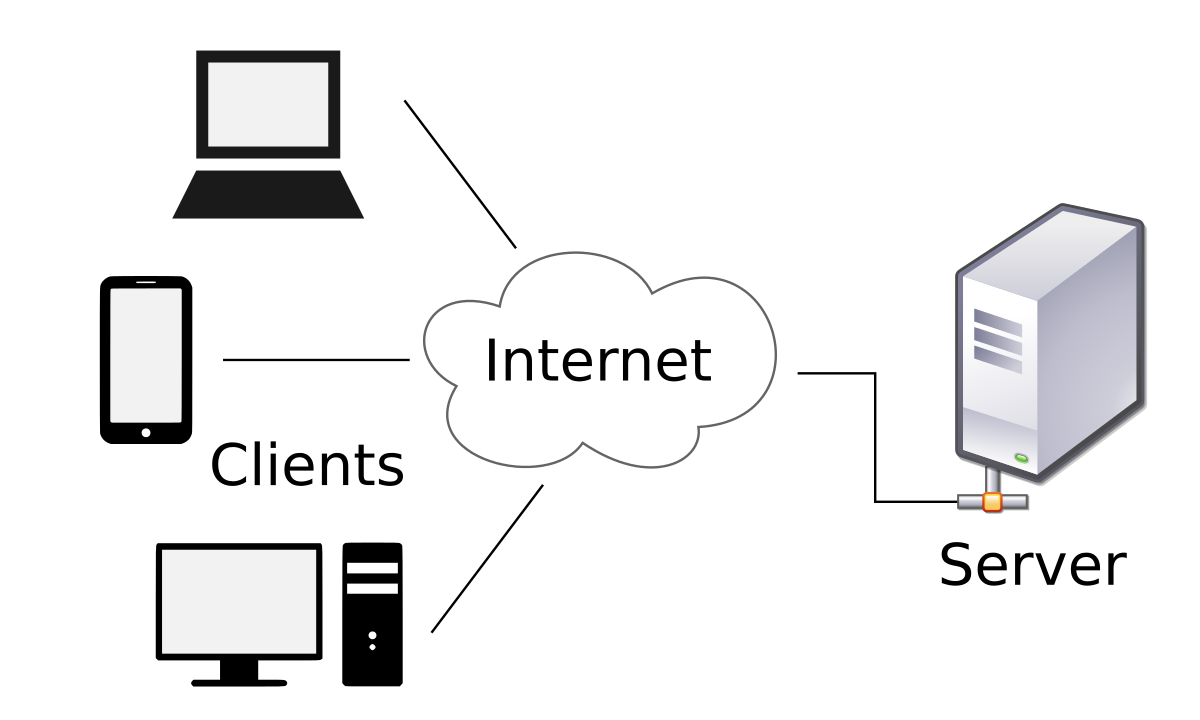
\includegraphics[width=0.8\textwidth]{figures/client-server-architecture.png}
\label{fig:client-server-architecture}
\end{figure}


\paragraph{} Web clients are merely software that communicate to a Web server by making requests. The communication is governed by HTTP. Web clients are often also referred to as user agents. A web browser is a particular type of user agent which acts on behalf of its user, i.e. acts as an agent, to satisfy their requests. There are other user agents, for example, command line tools that retrieve web page or other web resources using HTTP, but that don't render the results to the screen. For example, a web scraper or web indexer, is a user agent which collects web resources but does something else with them like, perhaps, building a database with the results. The reason we talk about web "clients" as well as user agents is because of the link to the client server architecture.
\paragraph{} To summarise, servers are software that responds to communications (HTTP requests) from clients (browsers).The response generally contains a document (HTML) that is transmitted back to the client as part of the response. Note that it can get (much) more complicated than that but this is a good starting place.


\section{Servers}
\paragraph{} The term server is heavily overloaded in computing. It can refer to hardware and it can also refer to software. Generally though we consider a server, whether hardware or software, to be acting in a particular role. That role is "serving", providing, or distributing data. Server software may run on server hardware, or might run incidentally on other hardware, for example, your laptop during development. Generally though we'll ignore the idea of server hardware in this module and just assume that on some level, all of our software is running somewhere appropriate. Server software isn't limited just to Web contexts though. For example, many database management systems work by using server software which responds to client requests. However a database, rather than speaking HTTP and HTML might instead use a query language like SQL or SPARQL. That said, some database servers also speak HTTP, an example of this is CouchDB which provides an API which can be accessed via a web browser. Whilst it's a little outside the scope of this module, it is worth considering just how many pieces of hardware out there could incorporate an HTTP server to provide a user interface to any browser rather than needing a specialised application. This is quite a democratising way to consider things and is especially exciting when we consider the idea of Internet of Things (IoT) and the notion that not only can the world provide data about what is happening to us, but things in the world can give us Web-based ways to interact with them.
\paragraph{} A server is, on the simplest interpretation, merely a piece of software that runs on a computer. It listens for messages and determines the right response to make (where the determination of request and response pairing is defined by the protocol).; we’ll l assume a server running on an Internet connected machine (so using TCP/ IP as lower level protocols). A web server is thus a server that listens for messages that are sent using web protocols (HTTP). By extension an email server is a server that listens for messages sent using email protocols (such as SMTP, IMAP, or POP).
\paragraph{} We've established that servers are responsive, they respond to something speaking to them by sending a message. If a server is listening then what is doing the speaking? 

\section{Web Clients \& User Agents}
\paragraph{} In the context of the Web, the software doing the speaking is the web client (or user agent). This is just another piece of software (nothing particularly special). Again, a web client just happens to speak HTTP but can initiate requests rather than merely waiting for them to arrive from other web clients. Other than this, a web client doesn't have to do anything more. It is useful to do something with the result of a request though. The result, the response, could just be logged, for example, the server responds with 200 OK. This would be enough if we were creating a web client that merely checked whether an HTTP server was alive and running correctly. A web spider (or search indexing agent) might retrieve pages from a site, then programmatically follow all the links to retrieve the pages that it links to and so on until it runs out of links to follow. Note that this is only a naive description of how a web spider might work. The spider would then do something else with the retrieved pages, perhaps building a database or analysing the page content for particular features. By contrast a web browser usually retrieves a single page then interprets the HTML content of the page to construct an internal, programmatic, representation of the page. This internal representation is the Document Object Model (DOM) which we will see soon. This DOM representation is then turned into, usually, graphical representation of the document. However, there are also text based browsers which manipulate the retrieved HTML document in a different way because they aren't visually based but are text oriented. Similarly a browser for the visually impaired might present an audio version of the page. The message to take away is that there is a lot more to the functionality of a web browser than merely retrieving pages and showing them to the user like a form of Internet PDF reader. Mobile apps are an increasingly popular web client. Frequently they will be retrieving data from a remote HTTP server (often as JSON documents rather than HTML documents) and then turning that data into a native application specific to the data retrieved rather than using a generic web browser. Essentially though, it is very easy for almost any piece of software to become a web client, it just needs to access, consume, or display web content, e.g. have the capability to talk usefully to an HTTP server.
\paragraph{} Let's now consider a specific type of web client, the web browser, possibly the most visible item of "web software" in our next topic.


\section{Web Browsers}
\paragraph{} Web browsers are software that not only speak HTTP so that they can retrieve HTML and other related documents from a web server but usually also contain some form of a layout engine that renders the web pages (HTML) into an appropriate form. This appropriate form is usually but not limited to the graphical web pages that we are used to from everyday web usage.
\paragraph{} The web browser is yet another invention from Berners-Lee. Having defined HTTP and HTML there was obviously a next step to create a user agent that could retrieve HTML from HTTP and then display it appropriately.
\paragraph{} Browsers are generally used to interactively navigate the public web but are also frequently used to access private networks, IoT interfaces, local file systems, and much more. 
\paragraph{} Browsers have also become a default cross-platform environment. Many items of software that might previously have been written as standalone desktop clients are now implemented as "web apps" that are generally accessible from any given web browser. This can solve many problems involved in the traditional development and distribution of software. For example, a new version of the software only has to be published to the web server and when the browser refreshes the page the new software is deployed. No more downloading, double clicking and installing or package managers required. However this is at the expense of different behaviours between various browsers which can affect user experience. There are also different performance characteristics when dealing with browsers compared with native applications. Also, browsers have been designed primarily for displaying web pages, which are essentially documents, with a particular flow of information and internal structure. This is not the same as a general graphical interface toolkit as might be used to develop for the desktop.
\paragraph{} There are many different producers of web browsers and the illustration gives you some idea of the prevalence and popularity of the more common of the various browsers. Note that this isn't entirely accurate because many browsers can identify as different user-agents, e.g. Firefox describing itself as Chrome, usually for compatibility. This is behaviour that is user-controlled and leads to the statistics on browser usage being a little uncertain.


\begin{figure}[H]
\centering
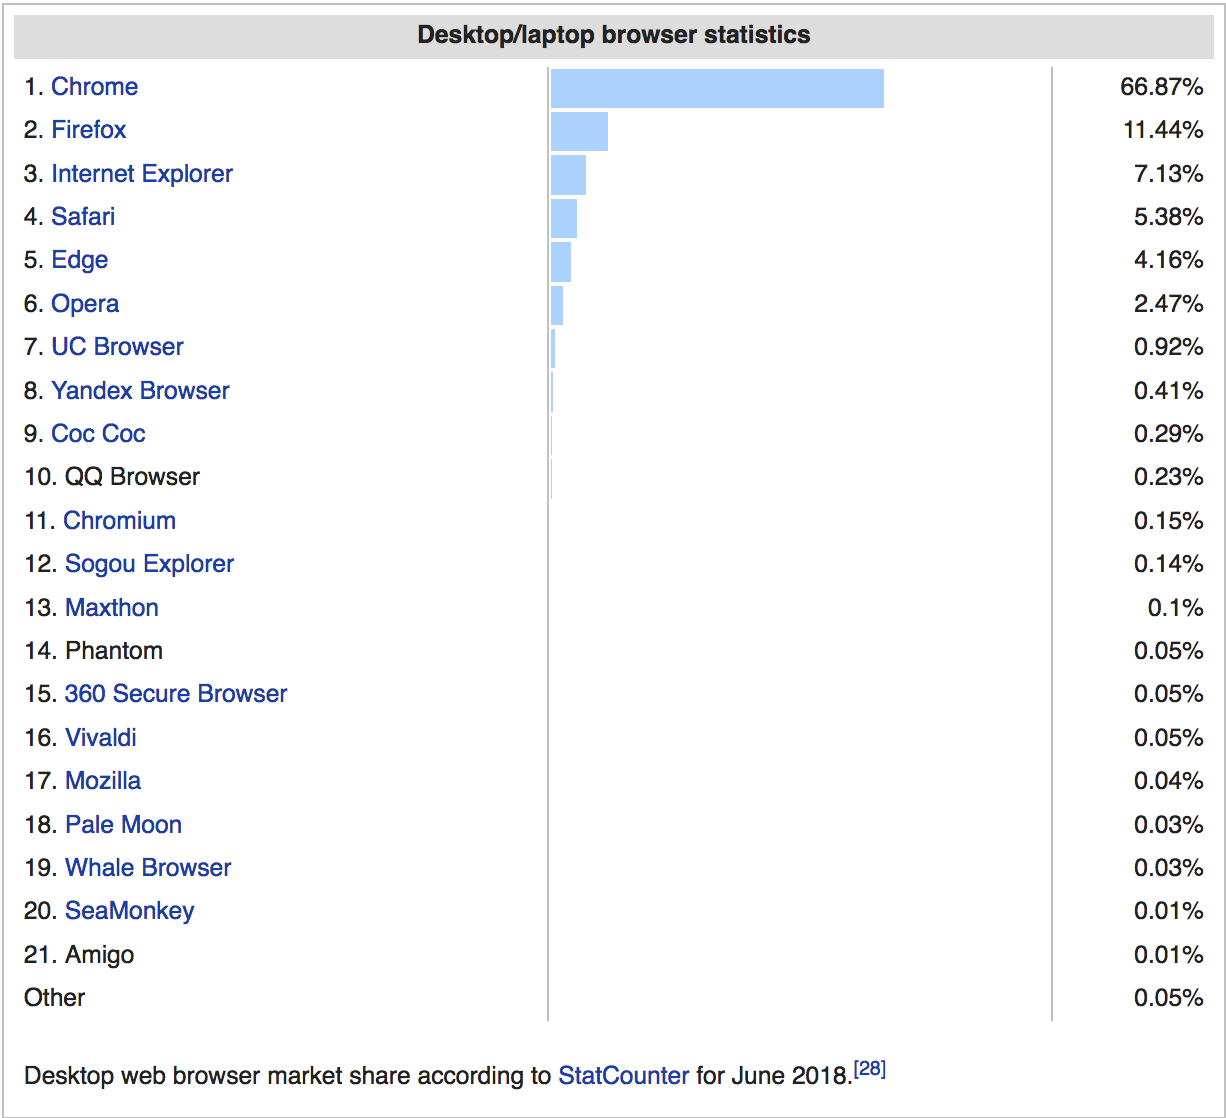
\includegraphics[width=0.8\textwidth]{figures/browser-stats.png}
\label{fig:browser-stats}
\end{figure}


\section{The Document Object Model (DOM)}
\paragraph{} We've made great progress now and have examined a lot of the technologies that are involved in retrieving a document from a web server and getting it into the browser. But what happens next?
\paragraph{} The HTML obviously needs to be altered from its default text based .html file into something that can be translated into the graphical display we are used to seeing in our web browsers. This is achieved by creating an intermediate model, named the Document Object Model (DOM).
\paragraph{} The DOM is a cross-platform, language independent Application Programming Interface (API). It parses the incoming HTML document, treating it as a tree data structure internally within your browser. The tree is formed due to the hierarchical and encapsulated nature of HTML tags where everything is enclosed within <html> tags at the top level. The <html> level encapsulates <head> and <body> tags which in turn encapsulates other tags, and so on, until everything is in place. This is heavily dependent upon the specific tags found in any given HTML document. HTML is parsed into this data structure to construct the DOM (for that document). Each part of this tree is represented internally to the browser as an object that can have various attributes and methods. These methods can then be called to manipulate the model, a process often referred to as manipulating the DOM. 
\paragraph{} The methods associated with the DOM provide an API that JavaScript can interact with to manipulate the current page. For example, Objects can be manipulated programmatically, e.g. using Javascript, and the results displayed in the view pane of the user agent (browser). The browser also provides other APIs for interacting with the environment from JavaScript but the DOM is a good place to start.
\paragraph{} It is also worth noting that the DOM and the HTML sources are not the same. You cannot rely on the HTML that you loaded initially being a good representation of what you see in the browser or what is represented internally in the DOM. When the HTML is parsed it is used to construct the DOM, but this model can then be manipulated by any linked JavaScript and also manipulated visually, or even hidden, through CSS. If you right click on a page in your web browser and select "view source" then you will see the original HTML that was retrieved from the web server. If instead of view source, you load the browser development tools then you can use these to inspect and manipulate the DOM, if you compare the two then you might notice that the DOM is not always identical to the source HTML.
\paragraph{} You can find a little more about using the Chrome dev tools to inspect the DOM here:
	\url{https://developers.google.com/web/tools/chrome-devtools/dom/}
\paragraph{} We will return to consideration of the DOM throughout the HTML, CSS, and JS topics in subsequent units. An awful lot of client-side javascript involves manipulating the DOM.

\section{Browser Developer Tools}
\paragraph{} Our final topic for this unit is to consider turning all of this theory into practice. We only really need a good editor and a good browser to get started with client-side Web development - Web IDE’s are often overkill for simple development.
\paragraph{} There are many browsers: Chrome, Chromium, Firefox, Safari, Opera, IE/Edge - but for this module we will focus on Chrome so that we all have a consistent development and learning environment. I'd still suggest having other browsers installed though so that you can compare behaviour between them.

\paragraph{} All newer browsers have support for some set of developer tools. Common Features of Developer Tools include the following:
\begin{itemize}
\item HTML \& DOM viewers \& editors
\item Web page assets, resources, network information 
\item Profiling \& Auditing
\item JavaScript Debugging \& Console 
\end{itemize}

\paragraph{} Chrome is currently very popular but it also pioneers many new ideas and directions for the future of the Web.
\paragraph{} It is fast, stable, and feature rich. It also has many tools to support developers - get access to the surface (the web page) but also the internals of the browser and the web page/application. We can launch the developer tools by following the procedure in this screenshot:

\begin{figure}[H]
\centering
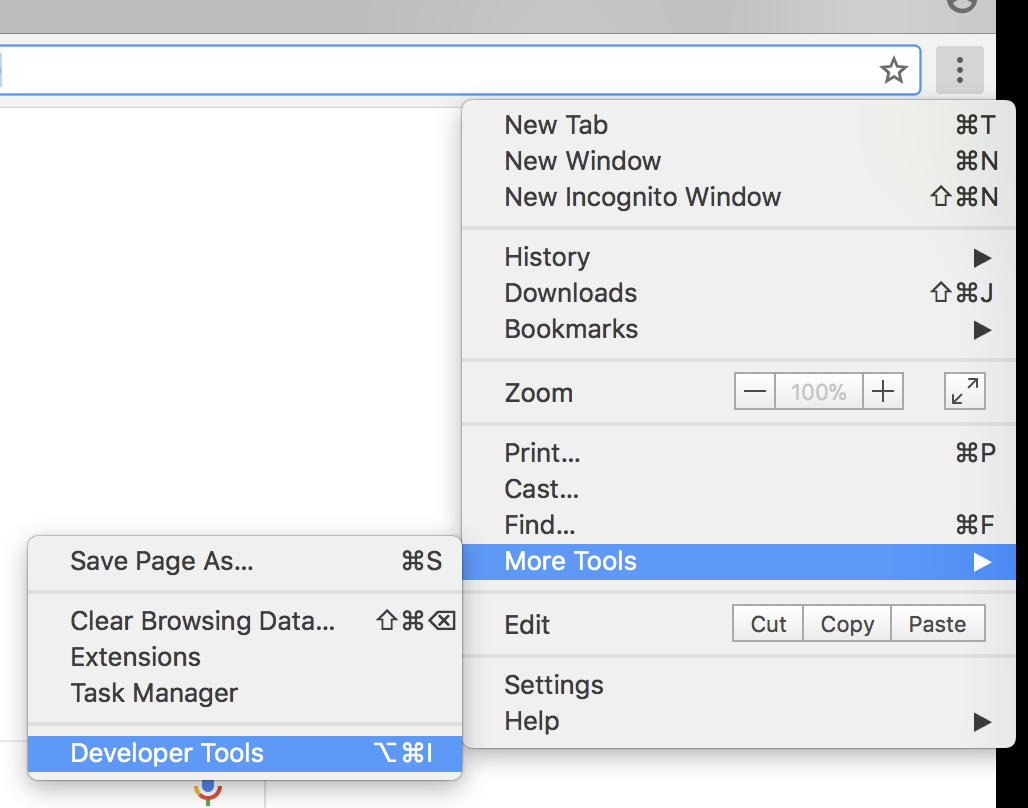
\includegraphics[width=0.8\textwidth]{figures/devtools.png}
\label{fig:devtools}
\end{figure}


\paragraph{} This gives us the following new set of tabs to interact with:

\begin{figure}[H]
\centering

\includegraphics[width=0.8\textwidth]{figures/devtools_toolbar.png}
\label{fig:devtools_toolbar}
\end{figure}


\paragraph{} For each tab we get a different view on aspects of the page that is loaded, for example the "elements" that is the DOM representation of the underlying HTML that the page is made up from. Note that this can become quite complicated because any associated CSS and Javascript can manipulate the HTML elements. As a result the HTML that is rendered in the browser for any given web page that you are viewing can be significantly different to the original HTML source file that was loaded. Remember this, CSS and JS give you great powers to manipulate a page, you can even discard all of the original HTML and completely generate a new replacement page.


\begin{figure}[H]
\centering
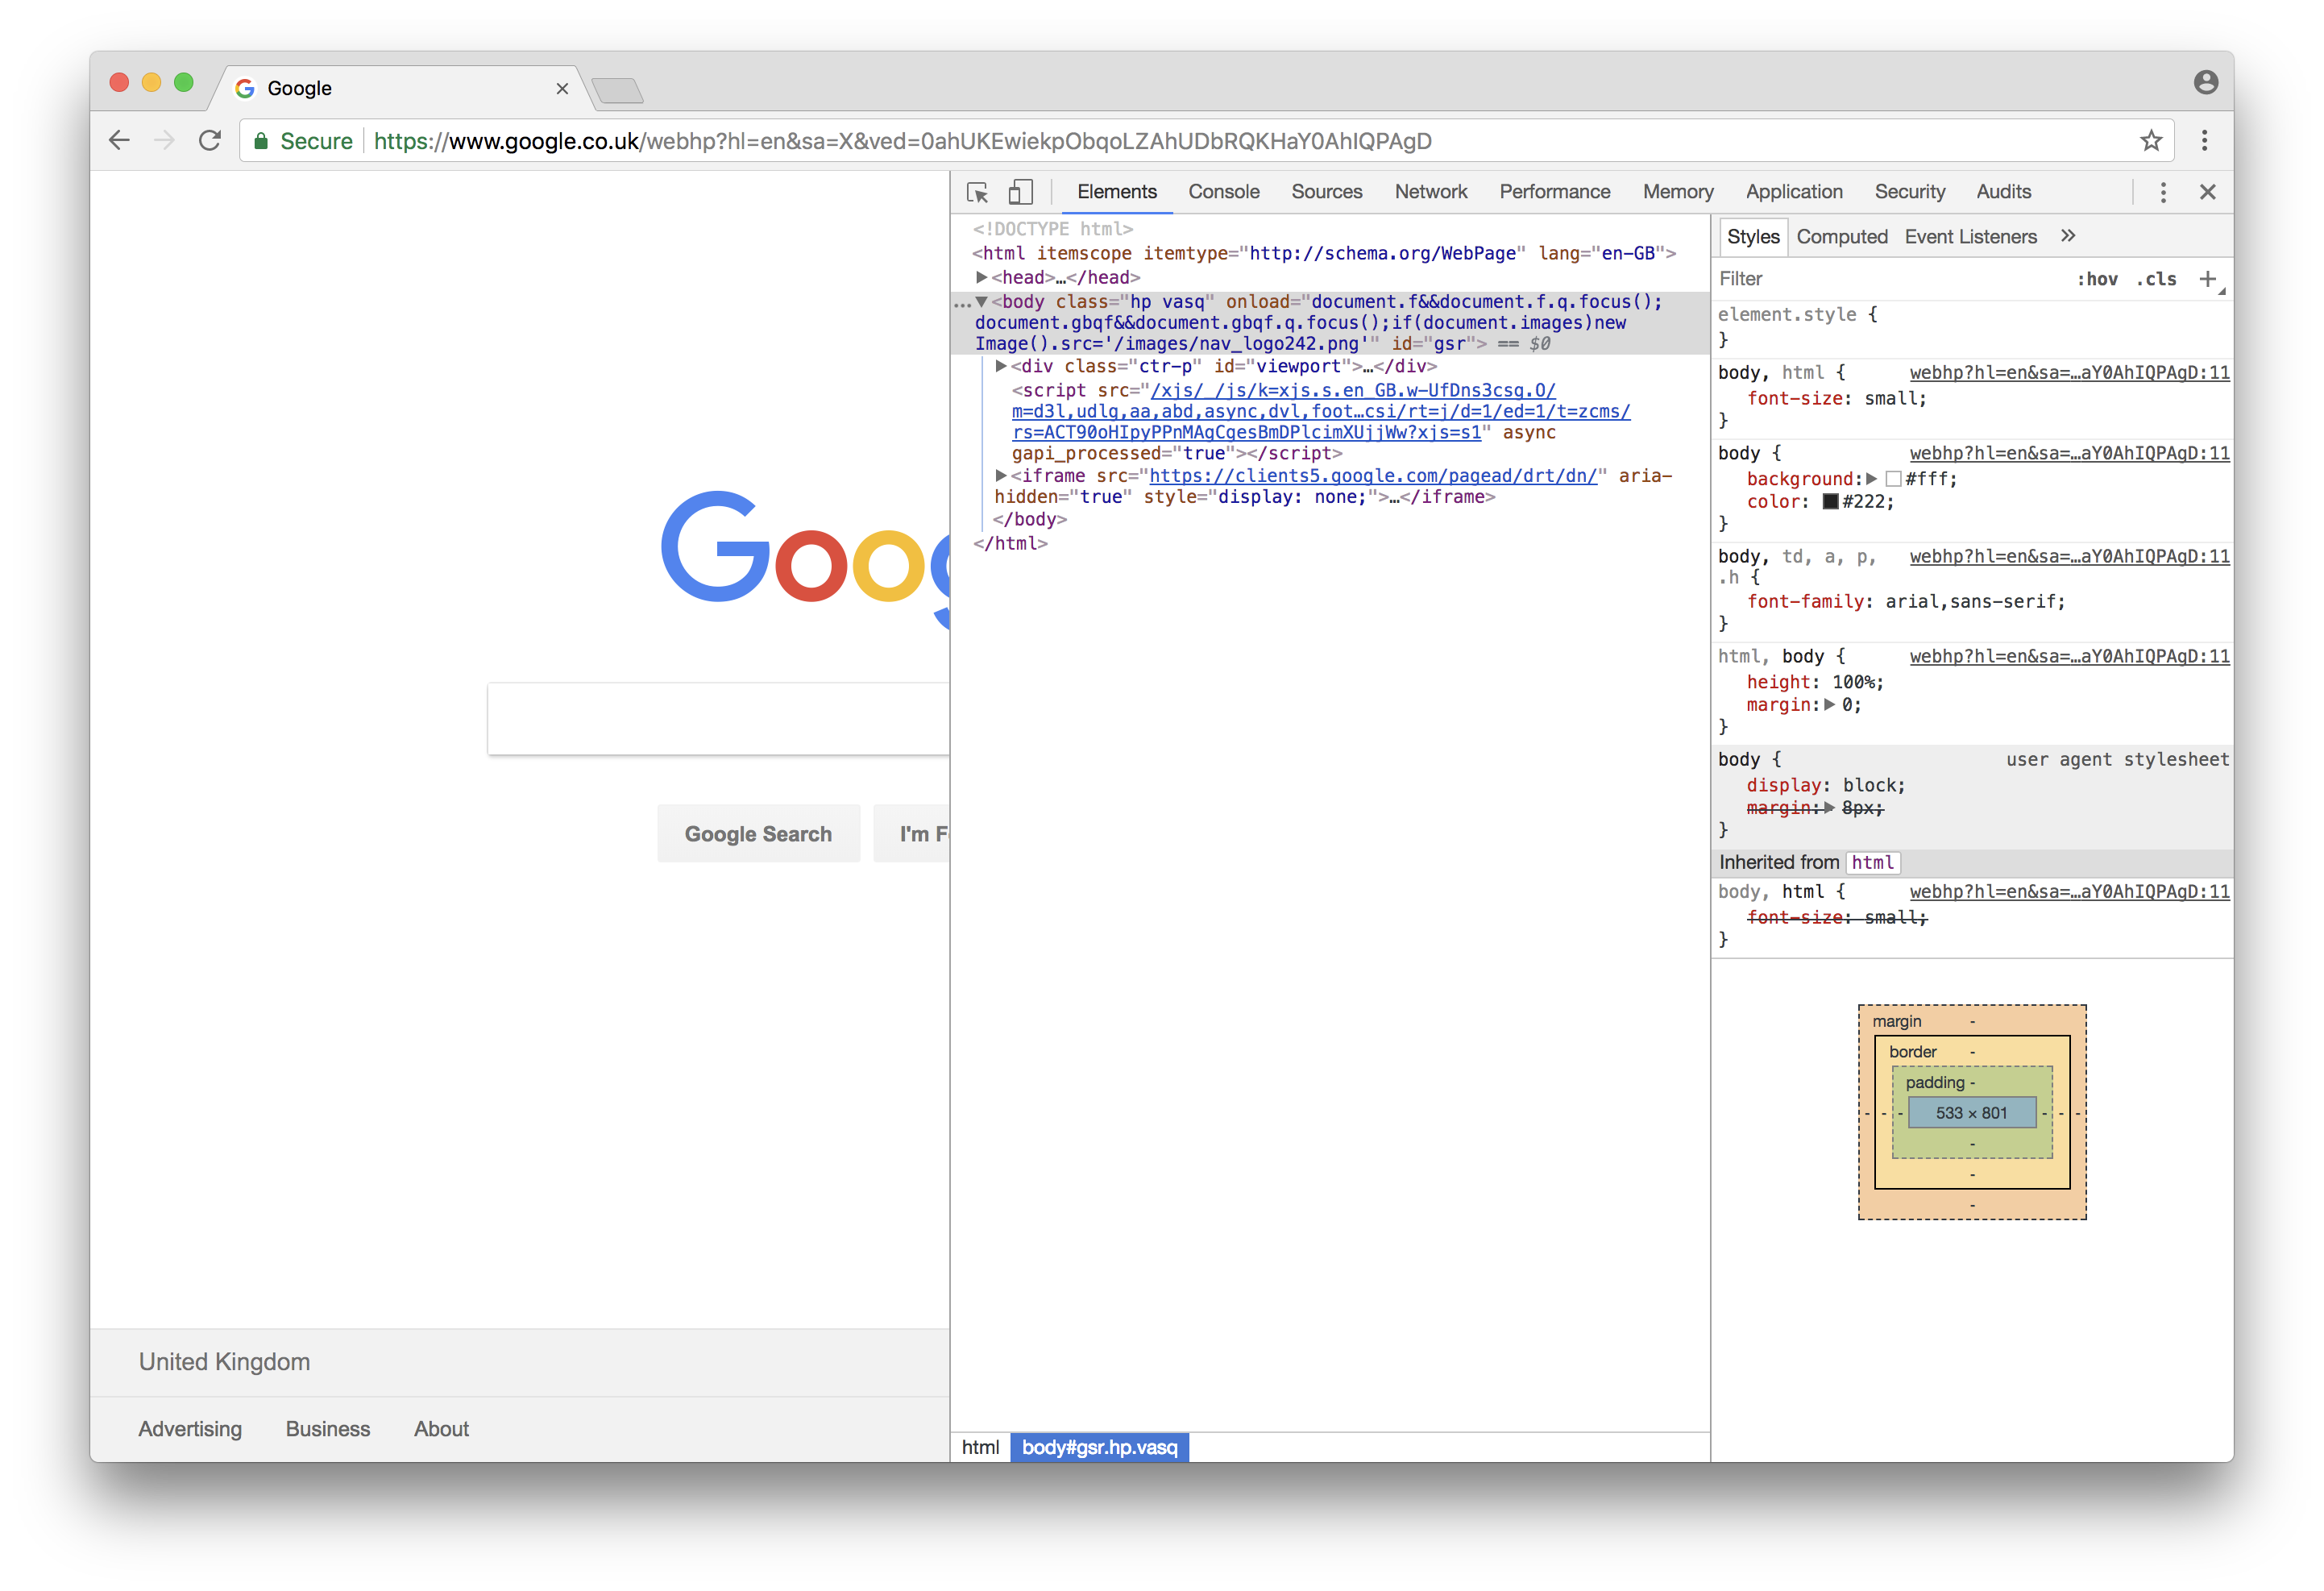
\includegraphics[width=0.8\textwidth]{figures/devtools_elements.png}
\label{fig:devtools_elements}
\end{figure}

\paragraph{} The next tab is for the console. This is a place that you will need to look at frequently as you develop your sites as it is the location where errors, warnings, and messages are printed when things go wrong.  You can also use it as a location to execute your own javascript. Just open the console and write some code then when you press return it will be executed. When you write more extensive JS in subsequent units you will find the console is a useful and important tool to have ready in your toolbox.


\begin{figure}[H]
\centering
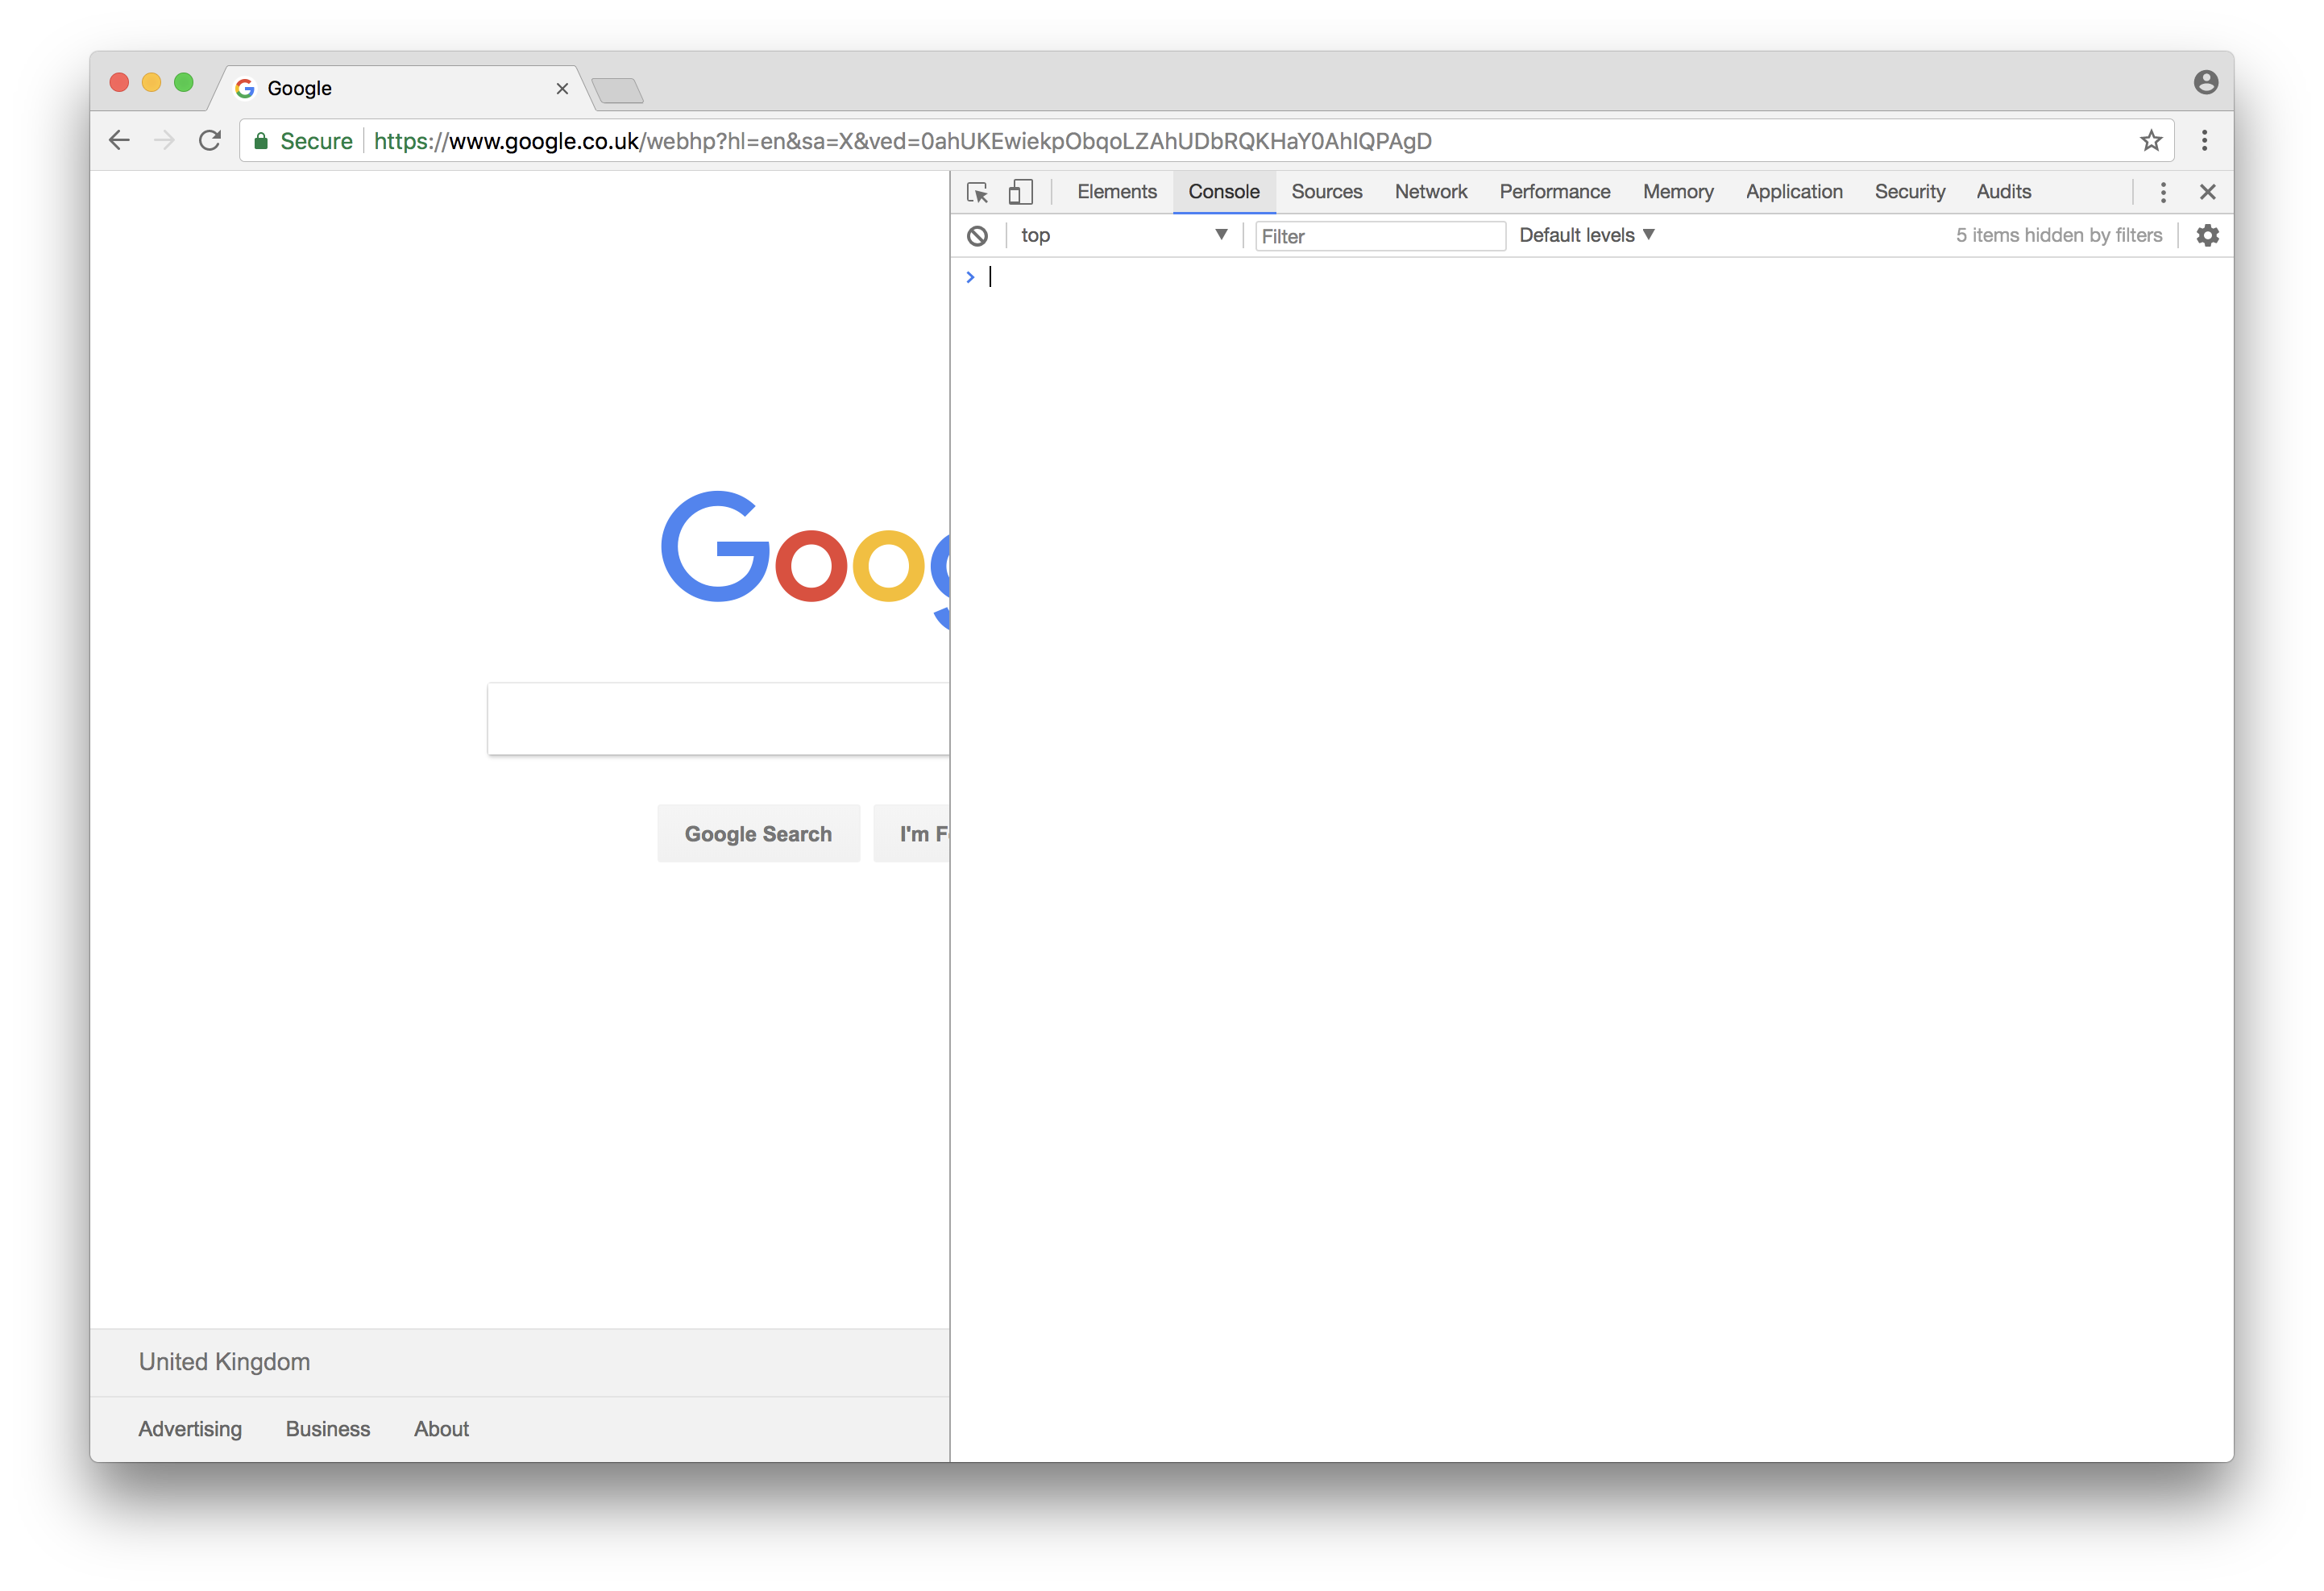
\includegraphics[width=0.8\textwidth]{figures/devtools_console.png}
\label{fig:devtools_console}
\end{figure}


\paragraph{} Next is the sources tab which will come in useful when we are dealing with deployed sites as it gives us a way to track all of the different resources that our pages use:


\begin{figure}[H]
\centering
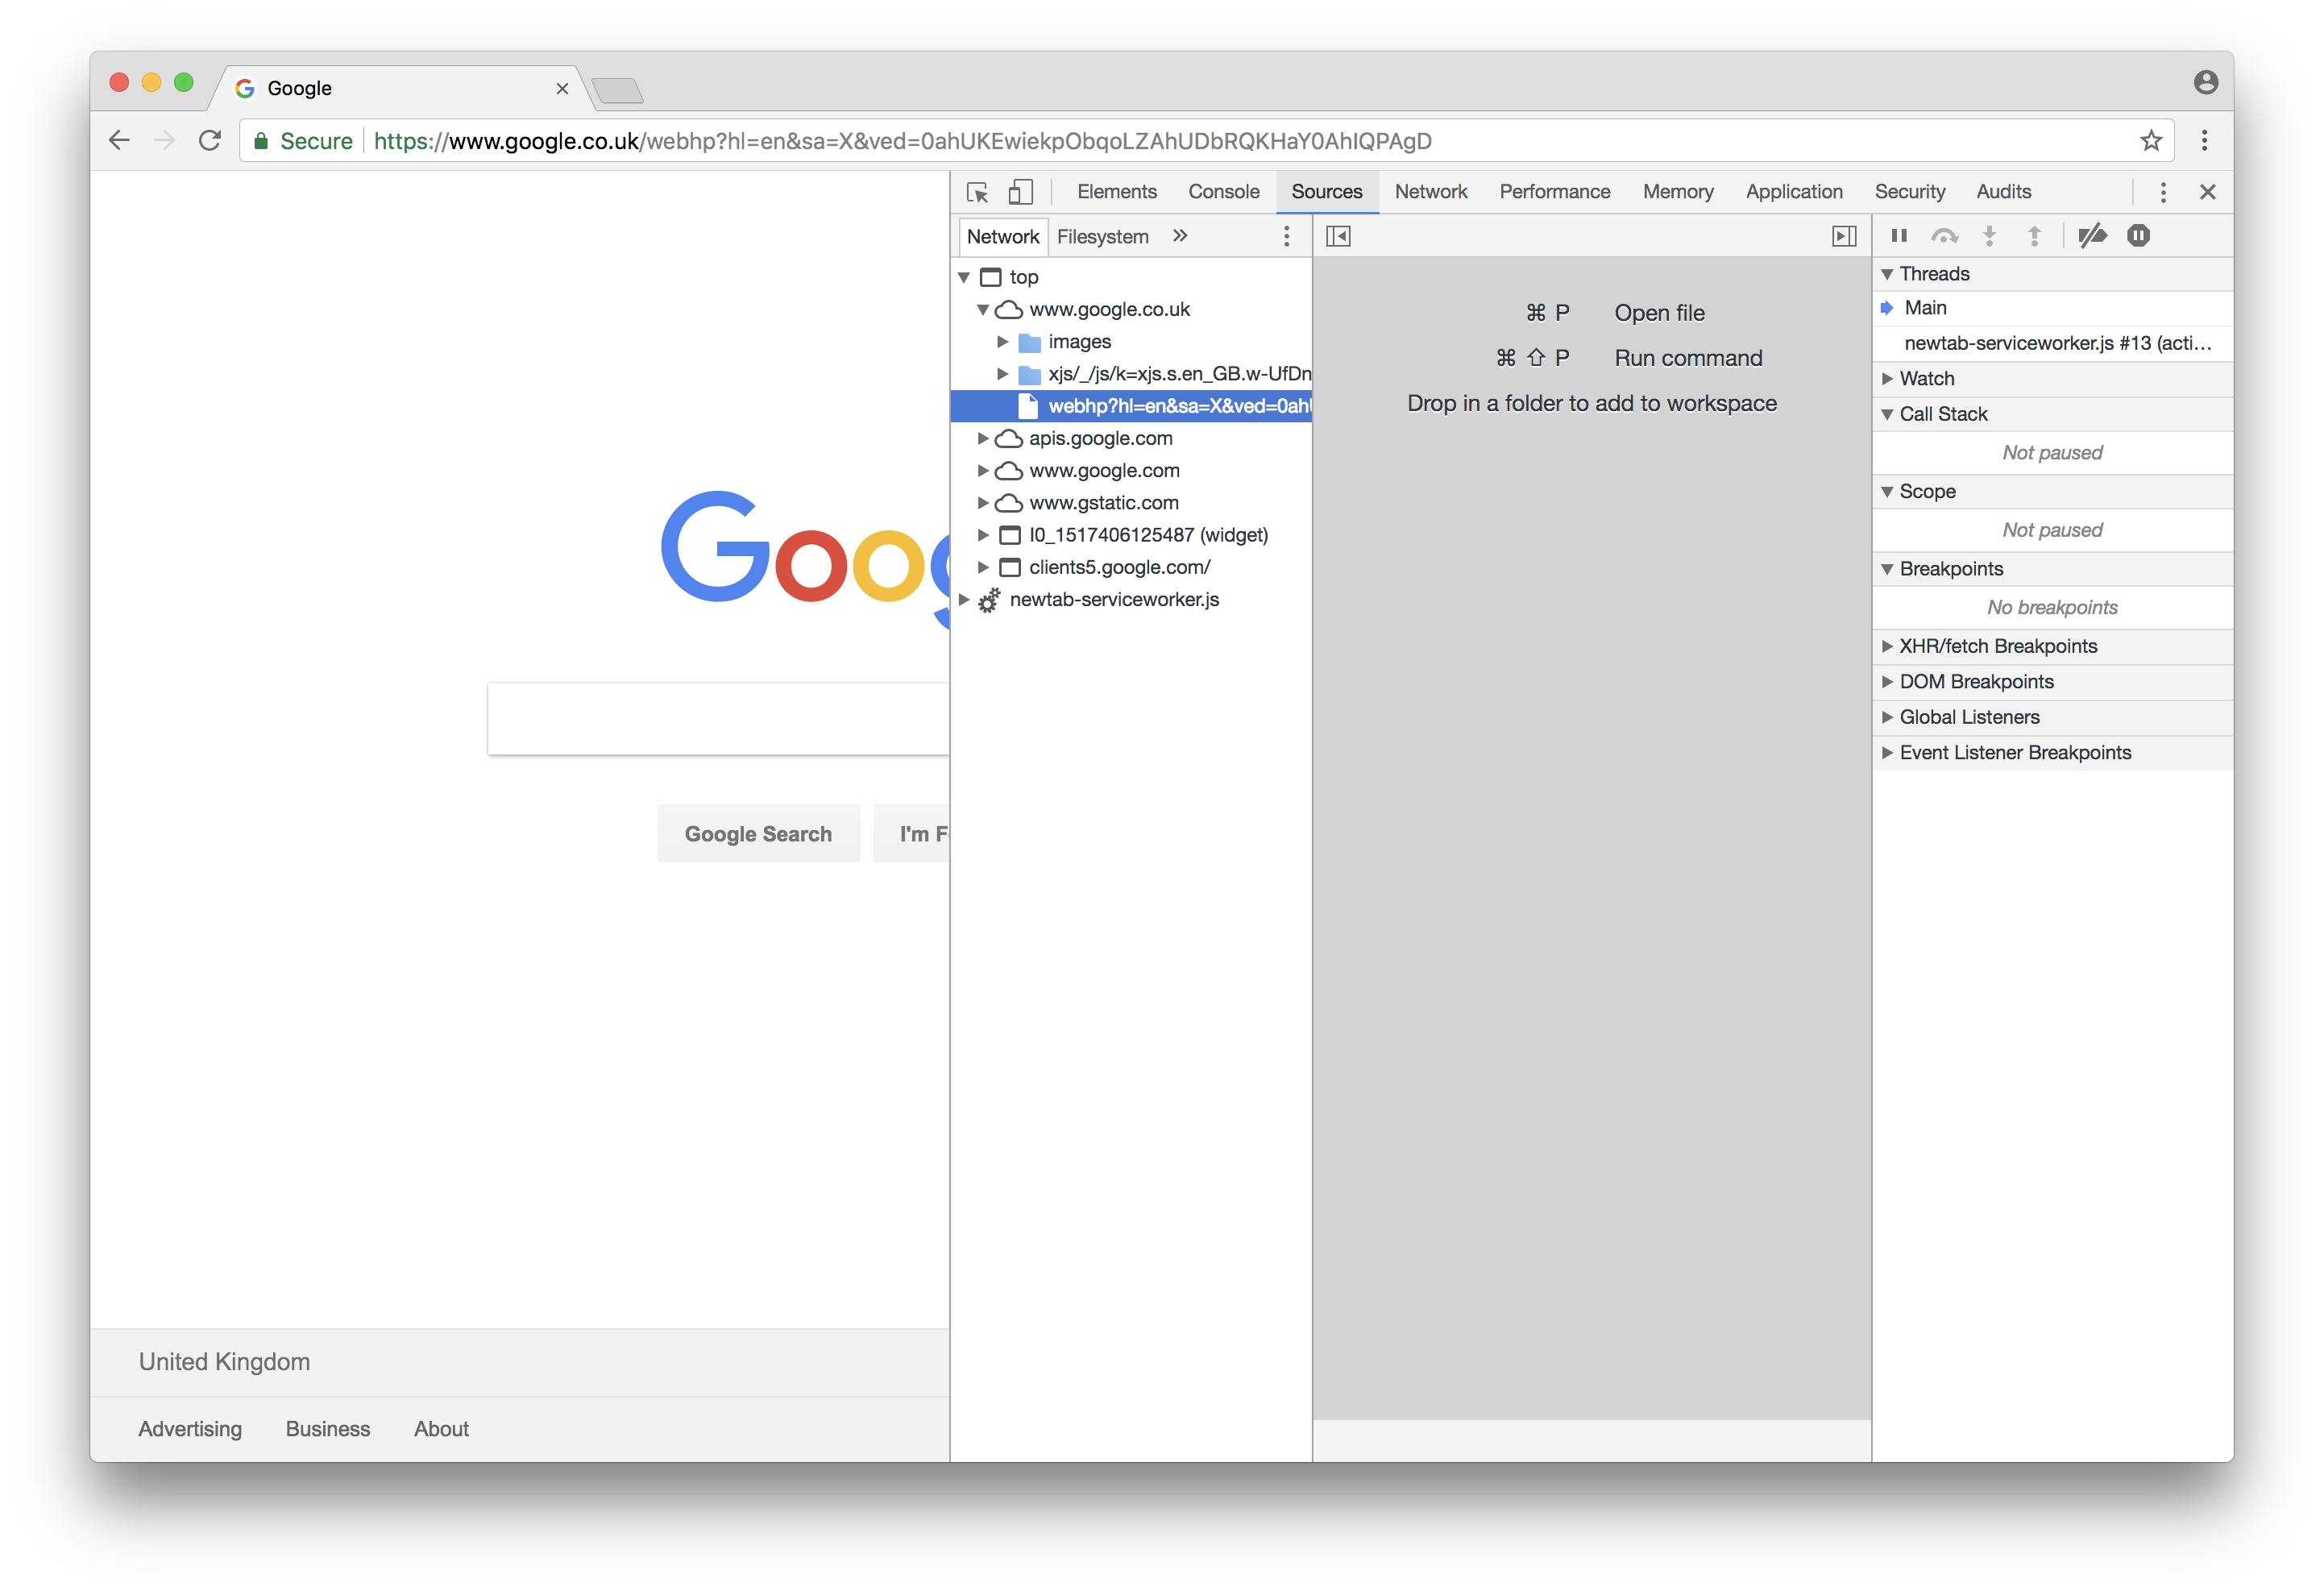
\includegraphics[width=0.8\textwidth]{figures/devtools_sources.png}
\label{fig:devtools_sources}
\end{figure}

\paragraph{} Our next tab, the network tab, gives us information about data and files being moved over the network/Internet/Web between your browser tab and all of the resources that the current web page is built from. This can be very useful when we build more complicated pages and need to debug why something isn't quite right.

\begin{figure}[H]
\centering
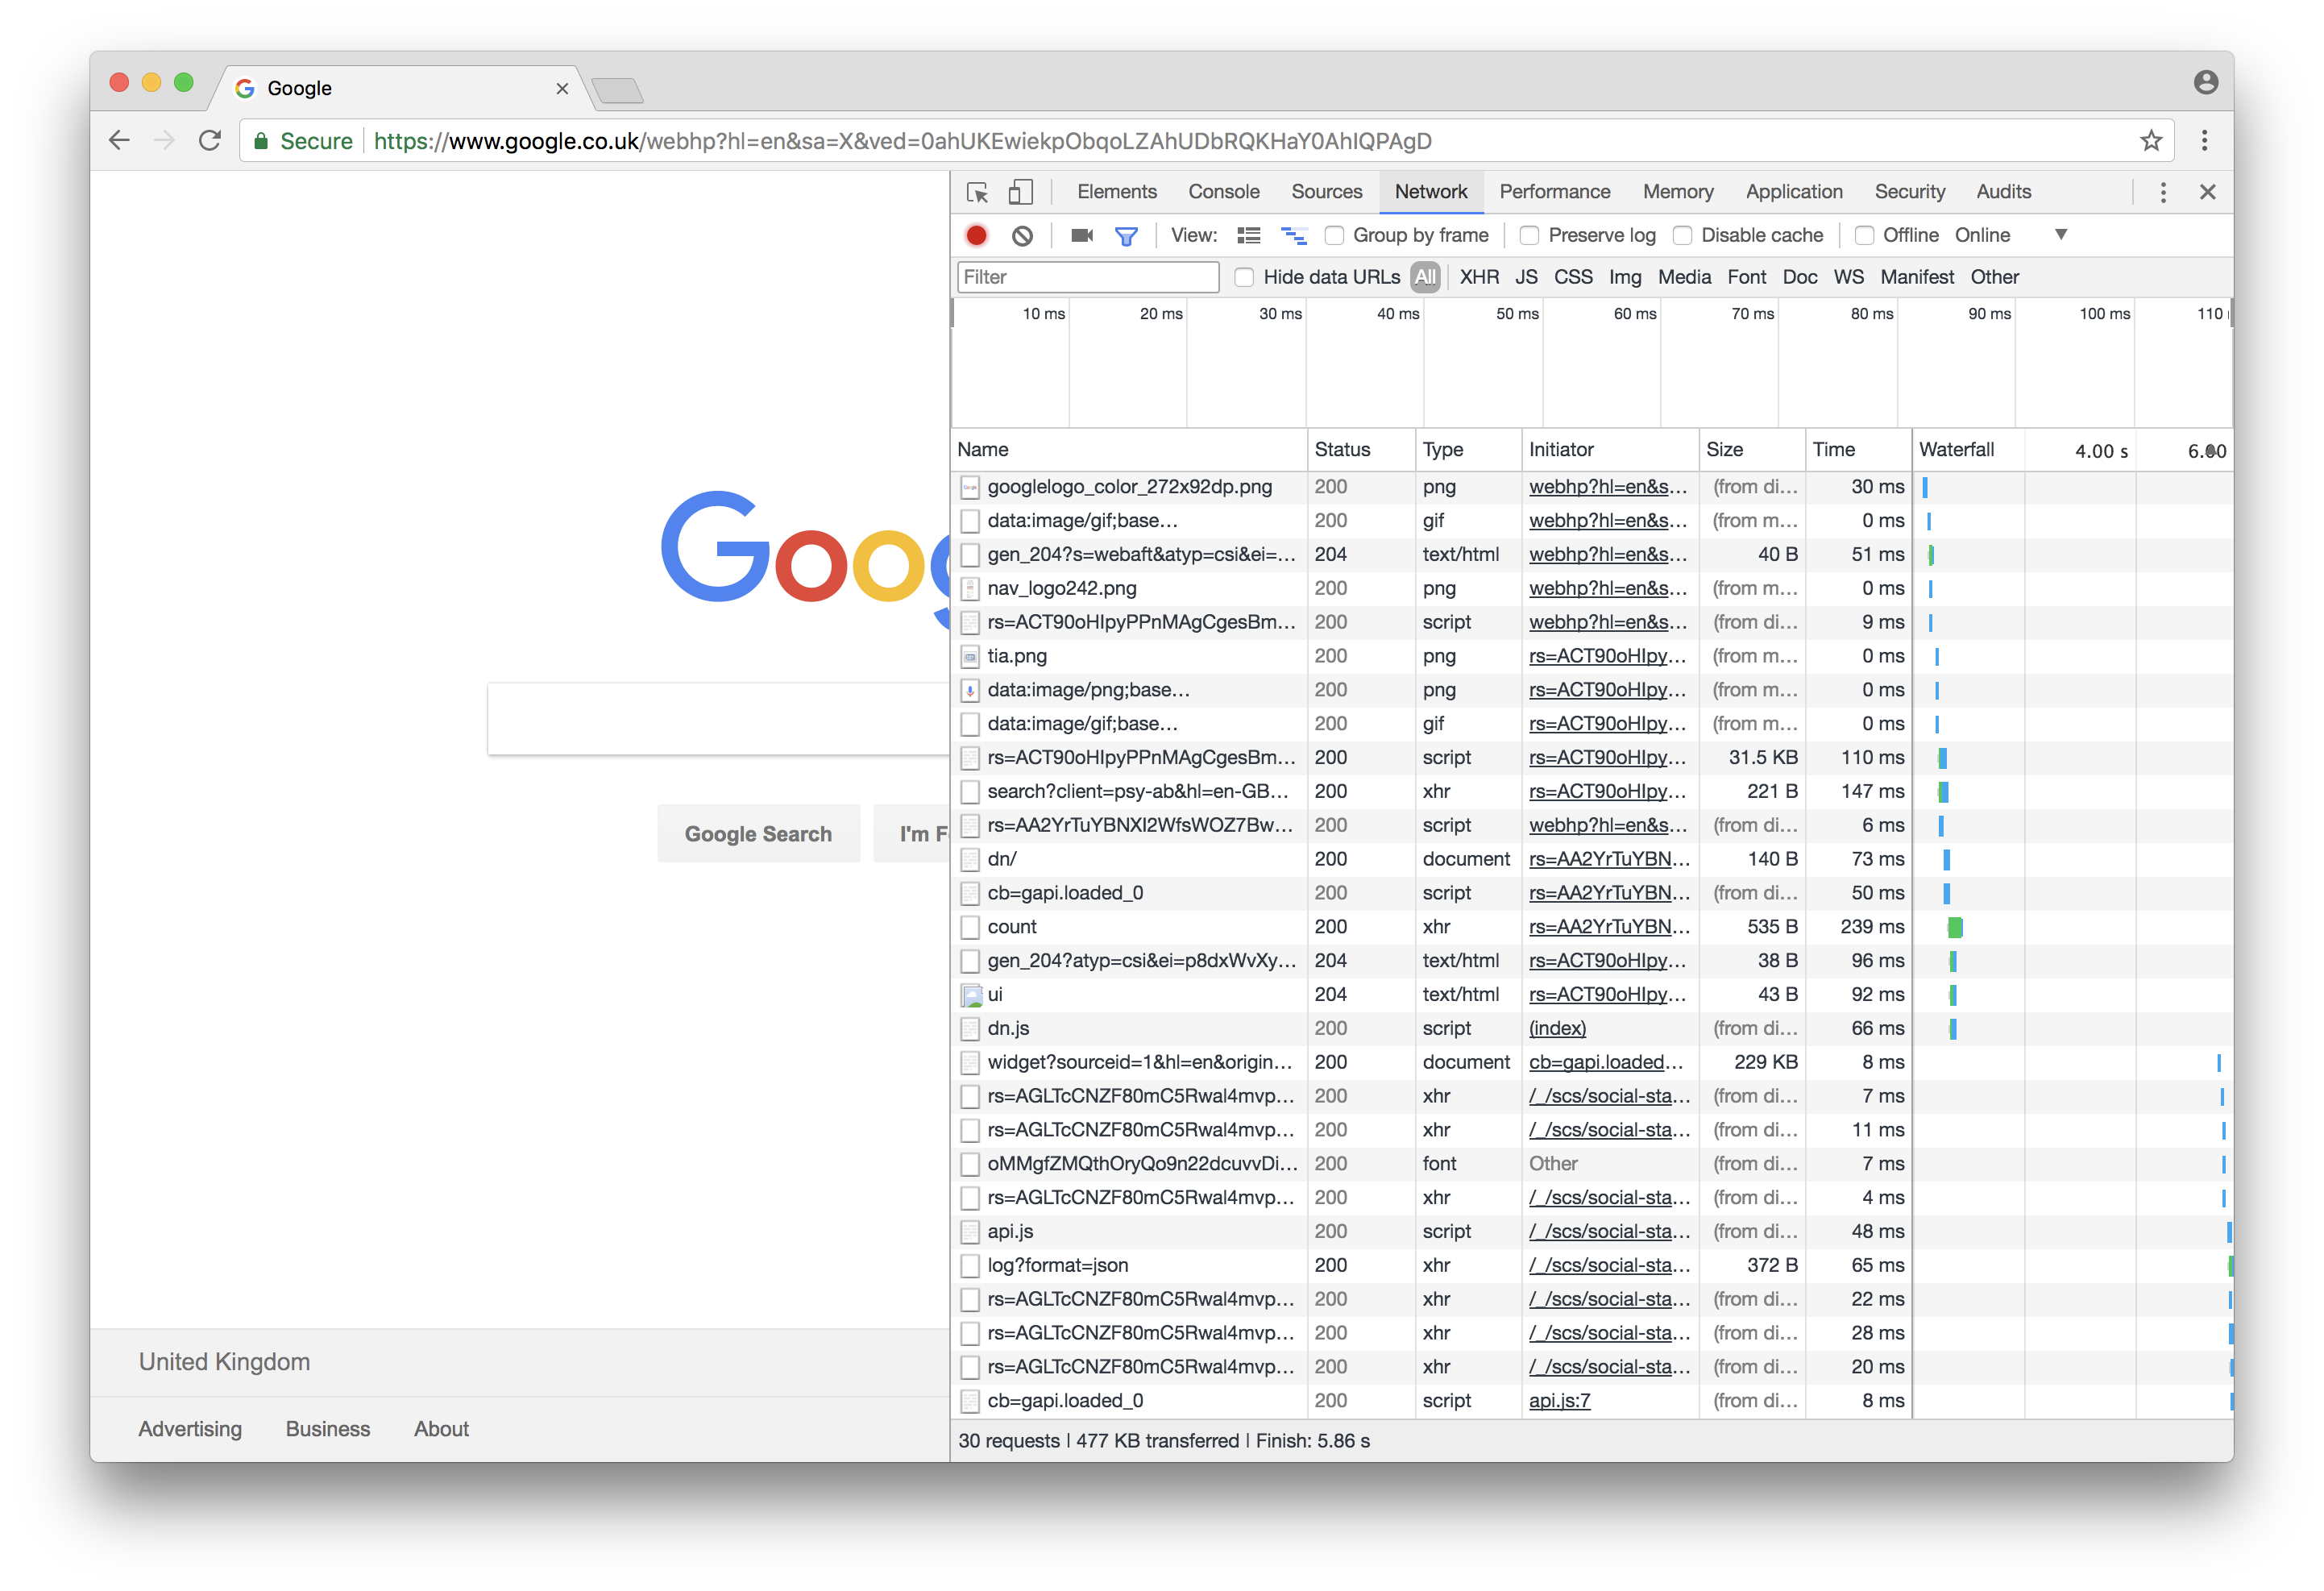
\includegraphics[width=0.8\textwidth]{figures/devtools-network.png}
\label{fig:devtools-network}
\end{figure}


\paragraph{} Next we have the performance monitor which we can use to inspect how well a page is working:

\begin{figure}[H]
\centering
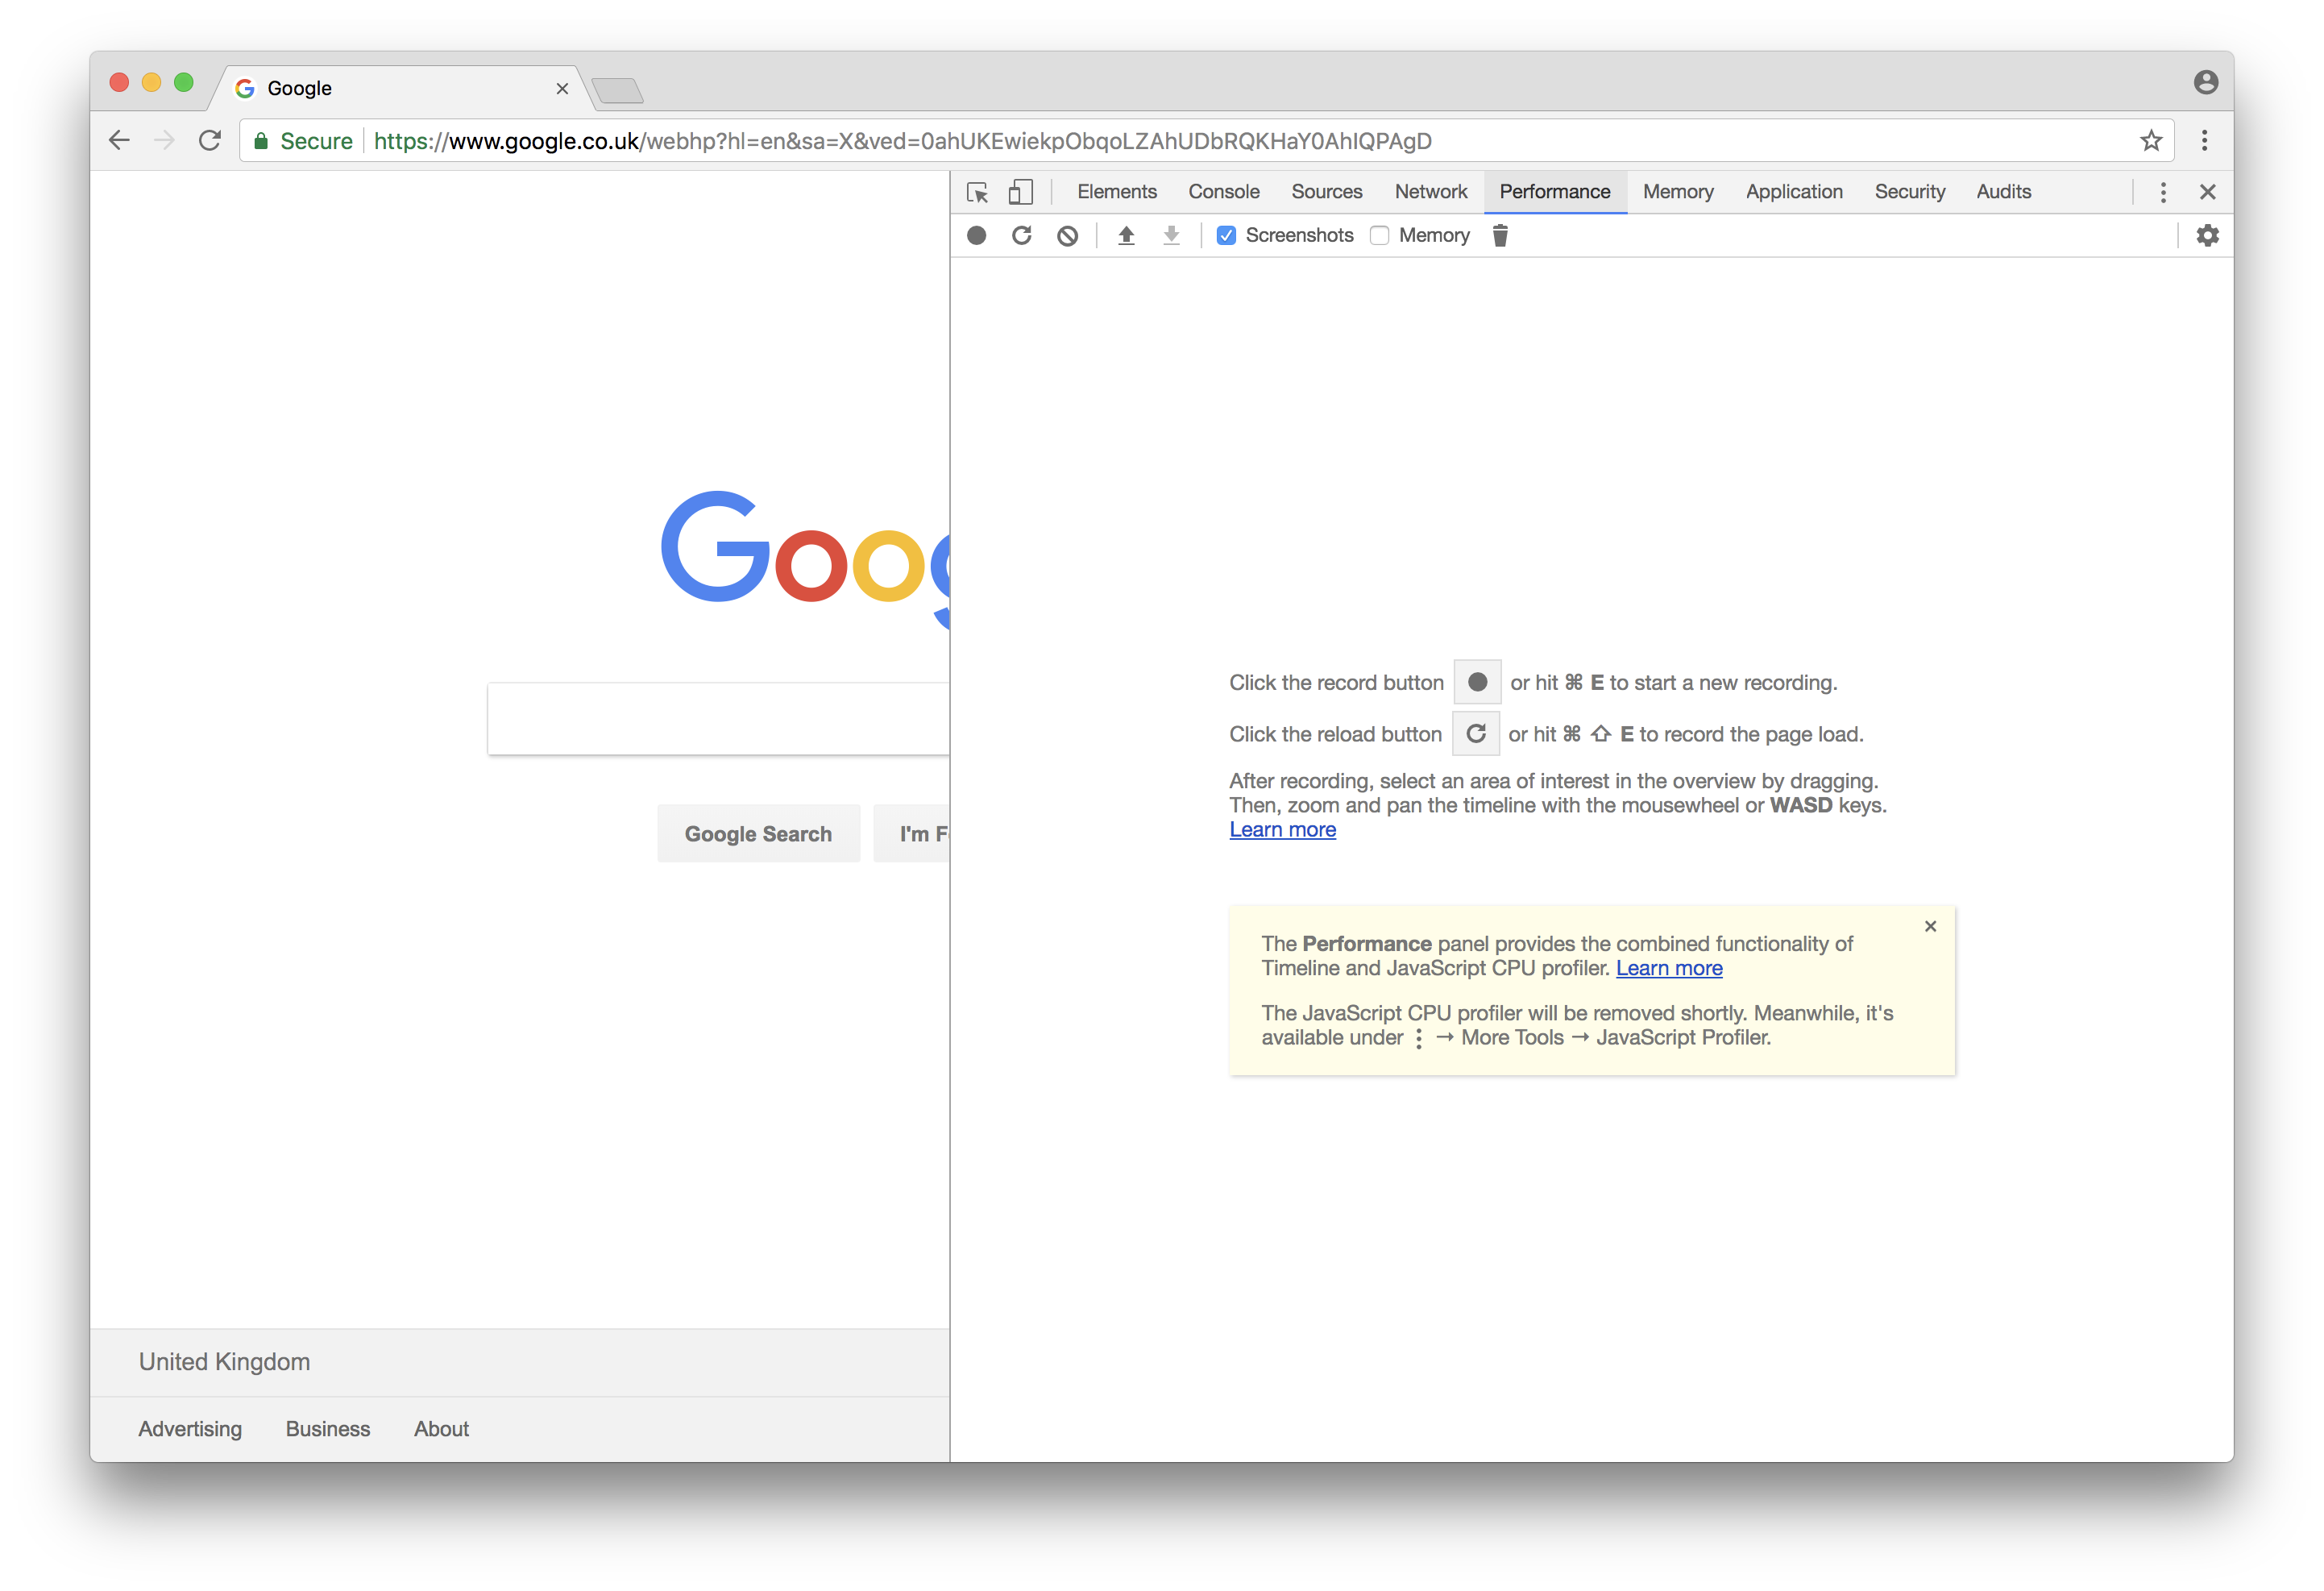
\includegraphics[width=0.8\textwidth]{figures/devtools-performance.png}
\label{fig:devtools-performance}
\end{figure}

\paragraph{} We can also profile memory usage which can be useful as start to write more extensive Javascript:

\begin{figure}[H]
\centering
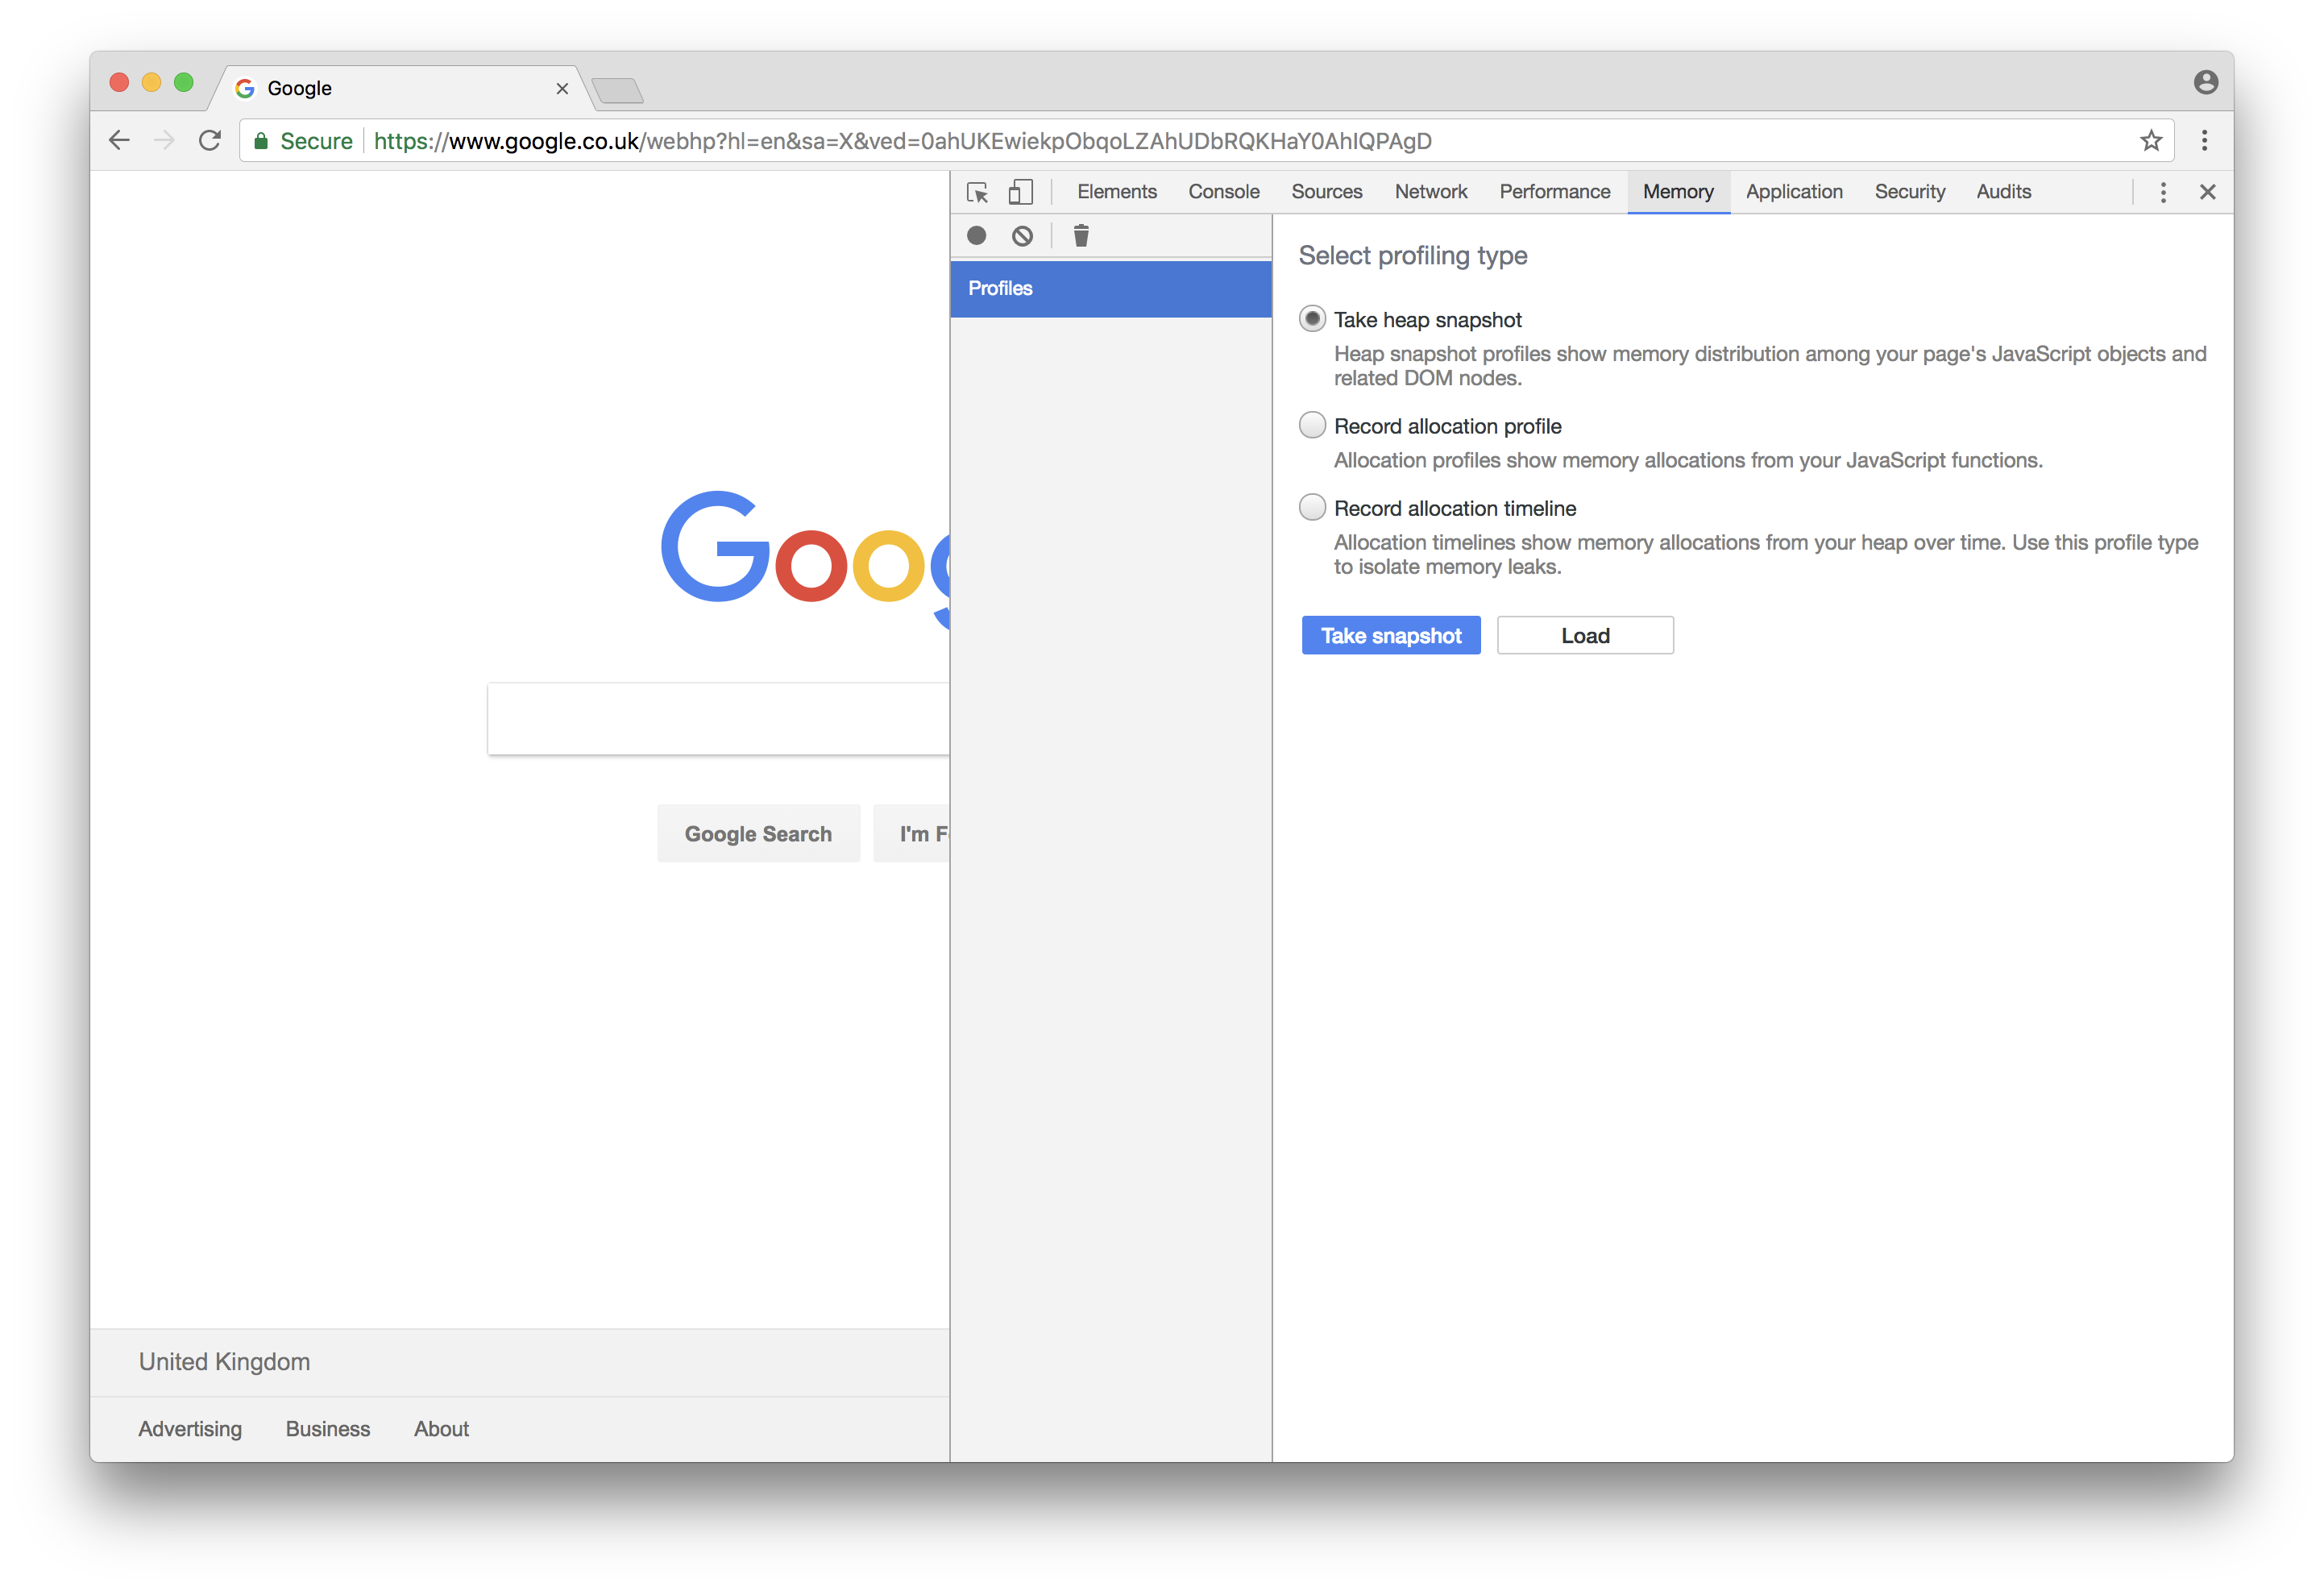
\includegraphics[width=0.8\textwidth]{figures/devtools-memory.png}
\label{fig:devtools-memory}
\end{figure}


\paragraph{} We can inspect aspects of the current web application, e.g. how local storage is being used, and which information is being cached:

\begin{figure}[H]
\centering
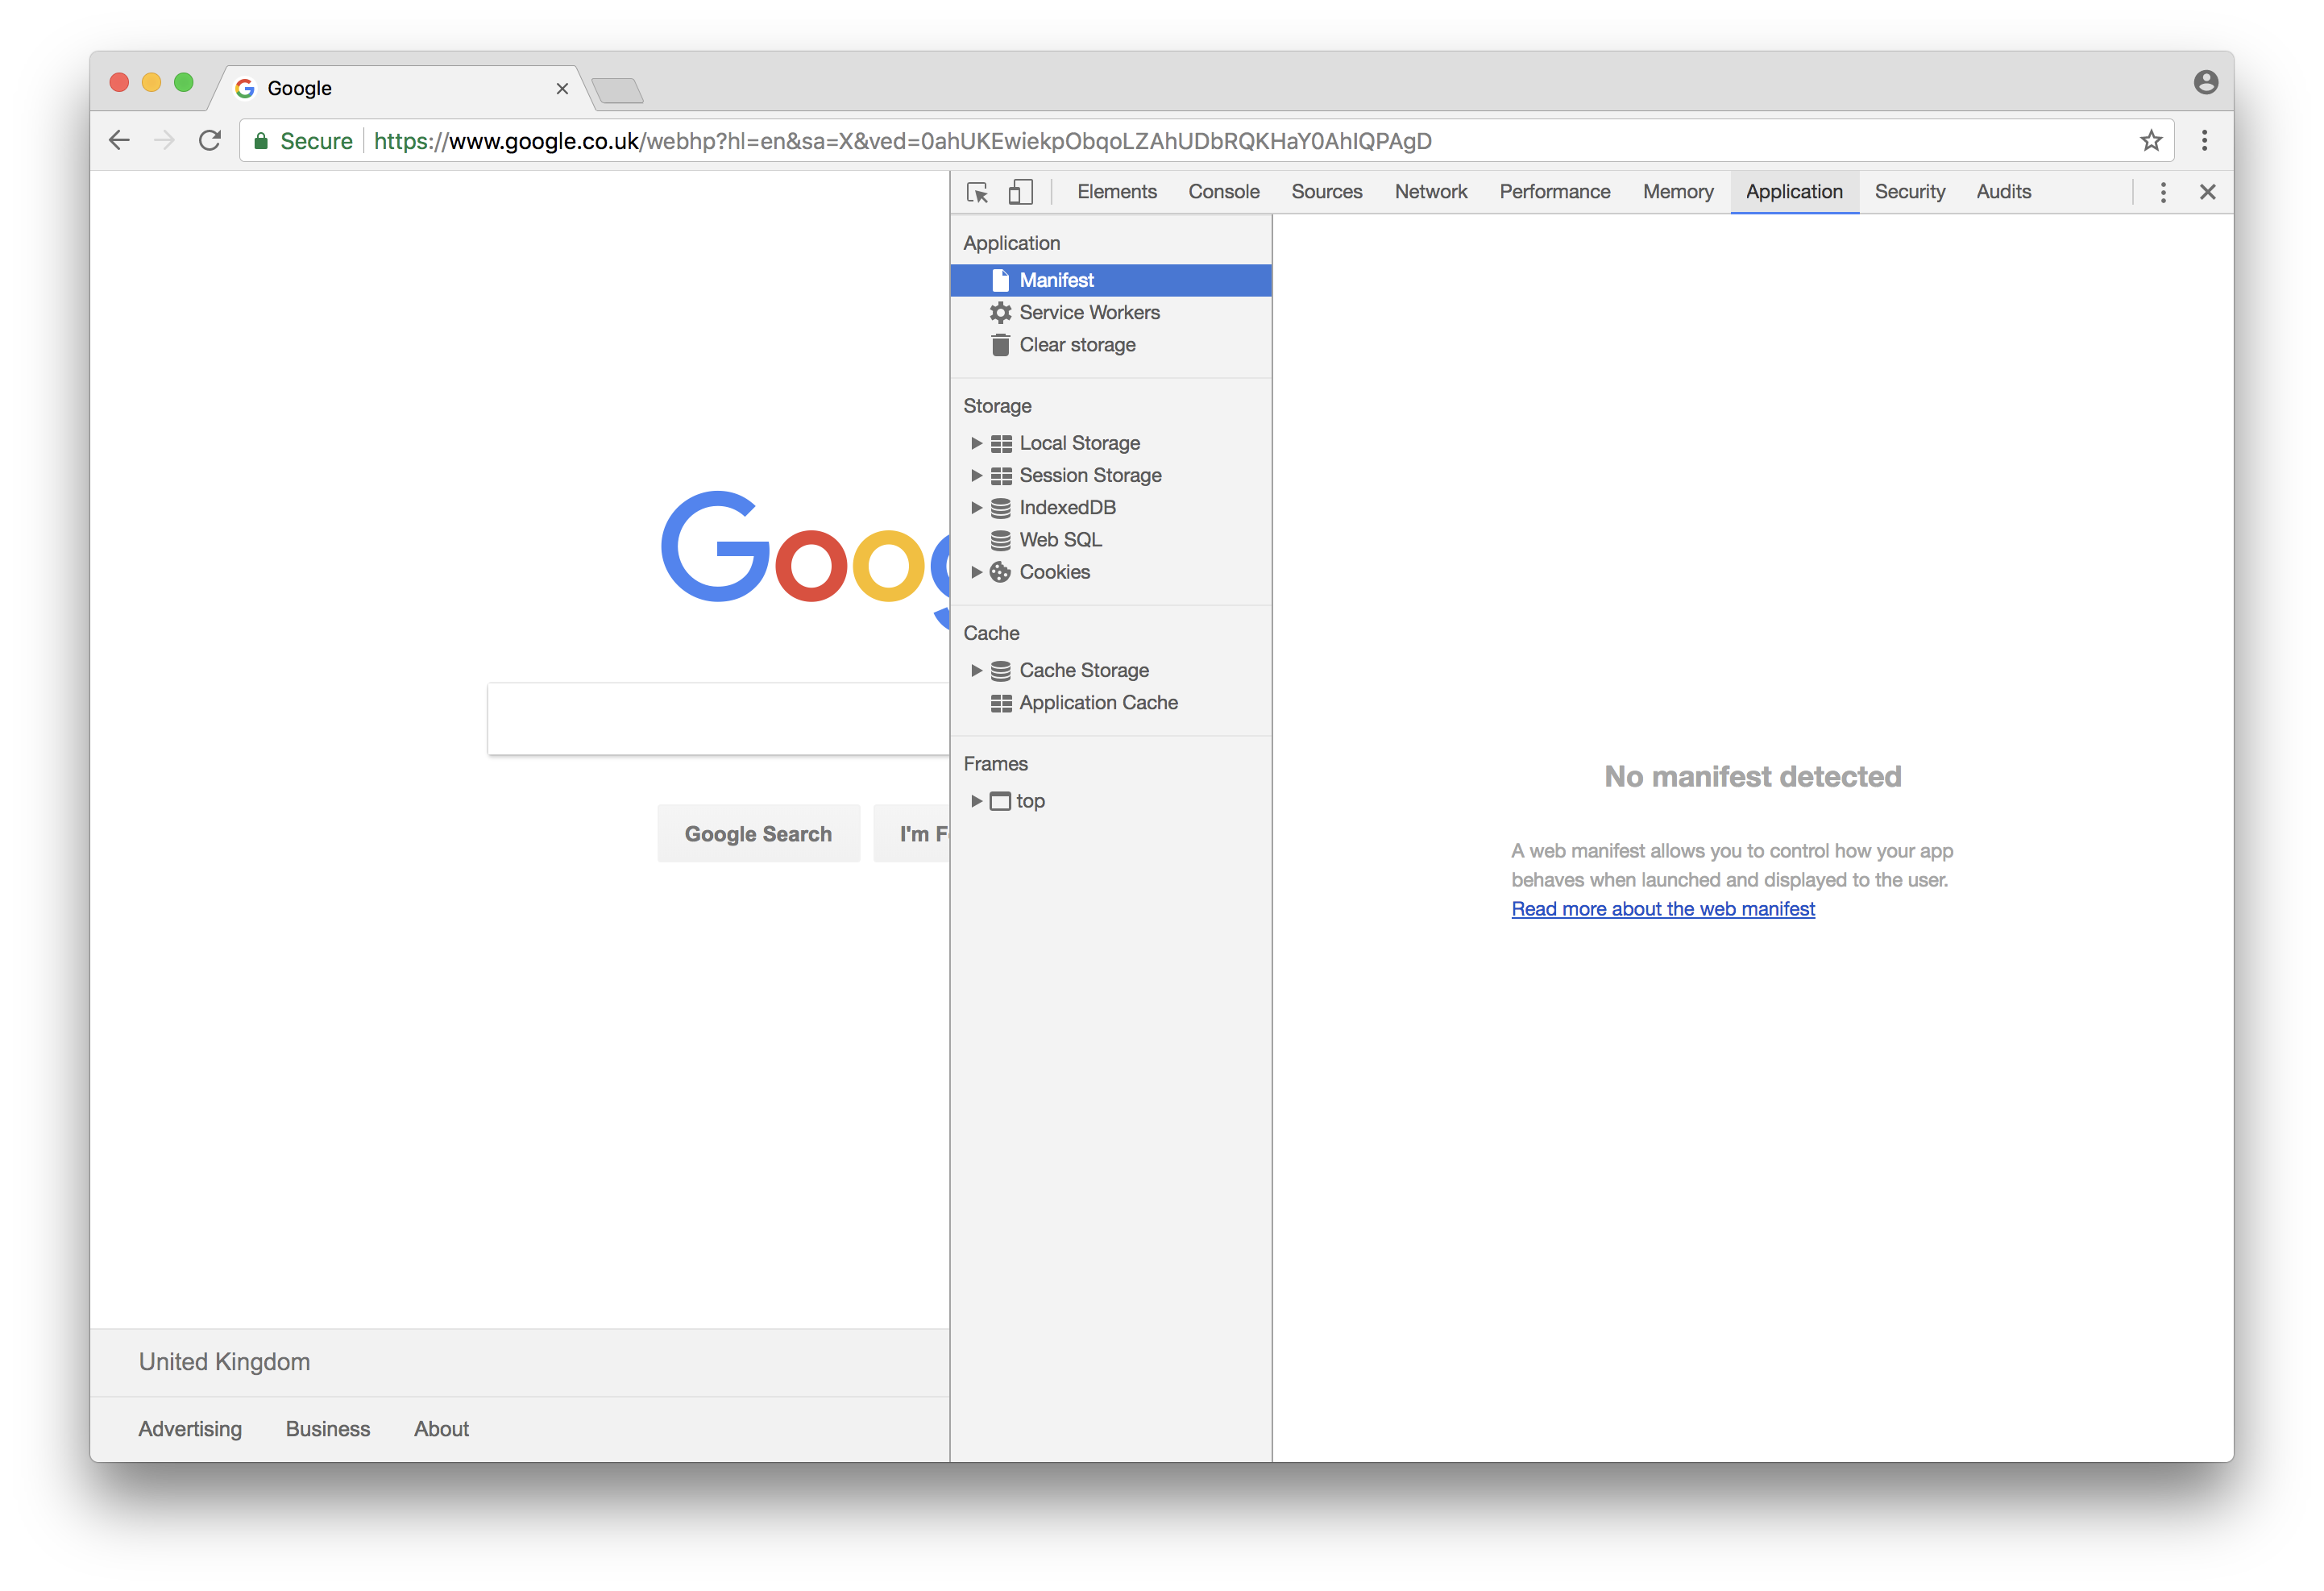
\includegraphics[width=0.8\textwidth]{figures/devtools-application.png}
\label{fig:devtools-application}
\end{figure}


\paragraph{} We can also inspect browser related security features:

\begin{figure}[H]
\centering
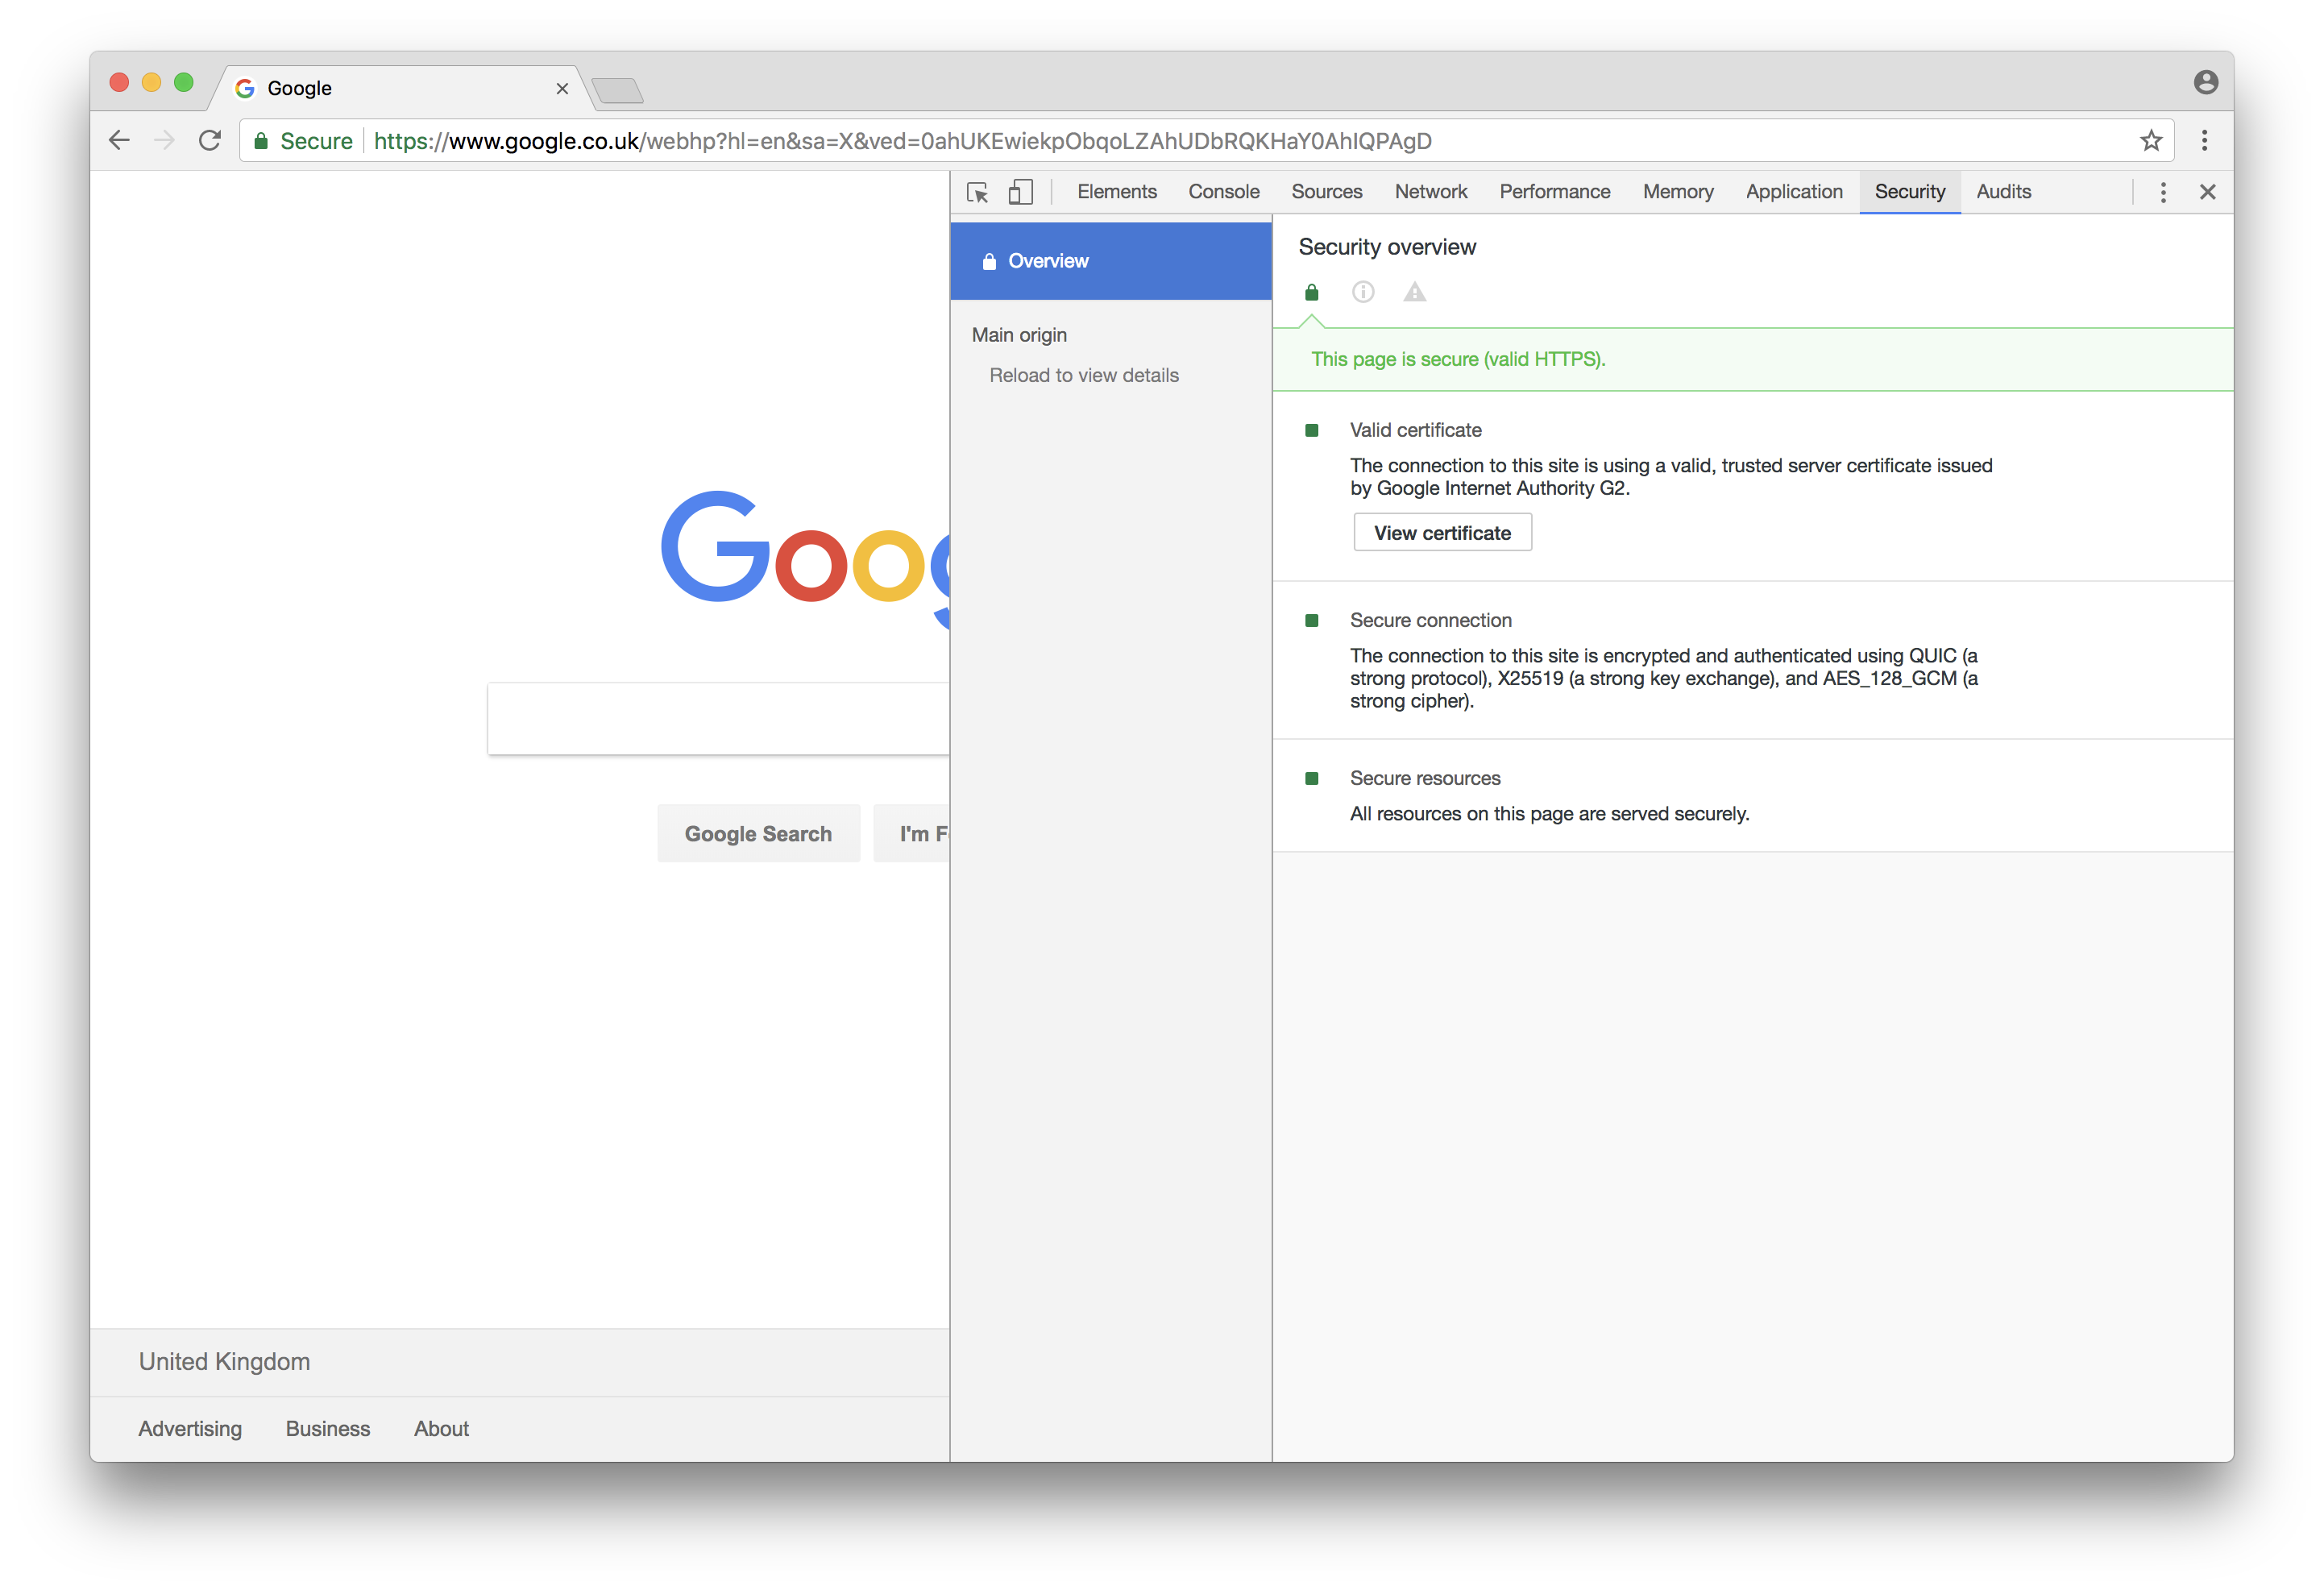
\includegraphics[width=0.8\textwidth]{figures/devtools-security.png}
\label{fig:devtools-security}
\end{figure}

\paragraph{} Finally, but no less important, Chrome supports an auditing feature using the Lighthouse project. This is a really useful tool for improving the quality of your pages. It audits against metrics for performance, accessibility, progressive web apps, search engine optimisation amongst many other aspects.

\begin{figure}[H]
\centering
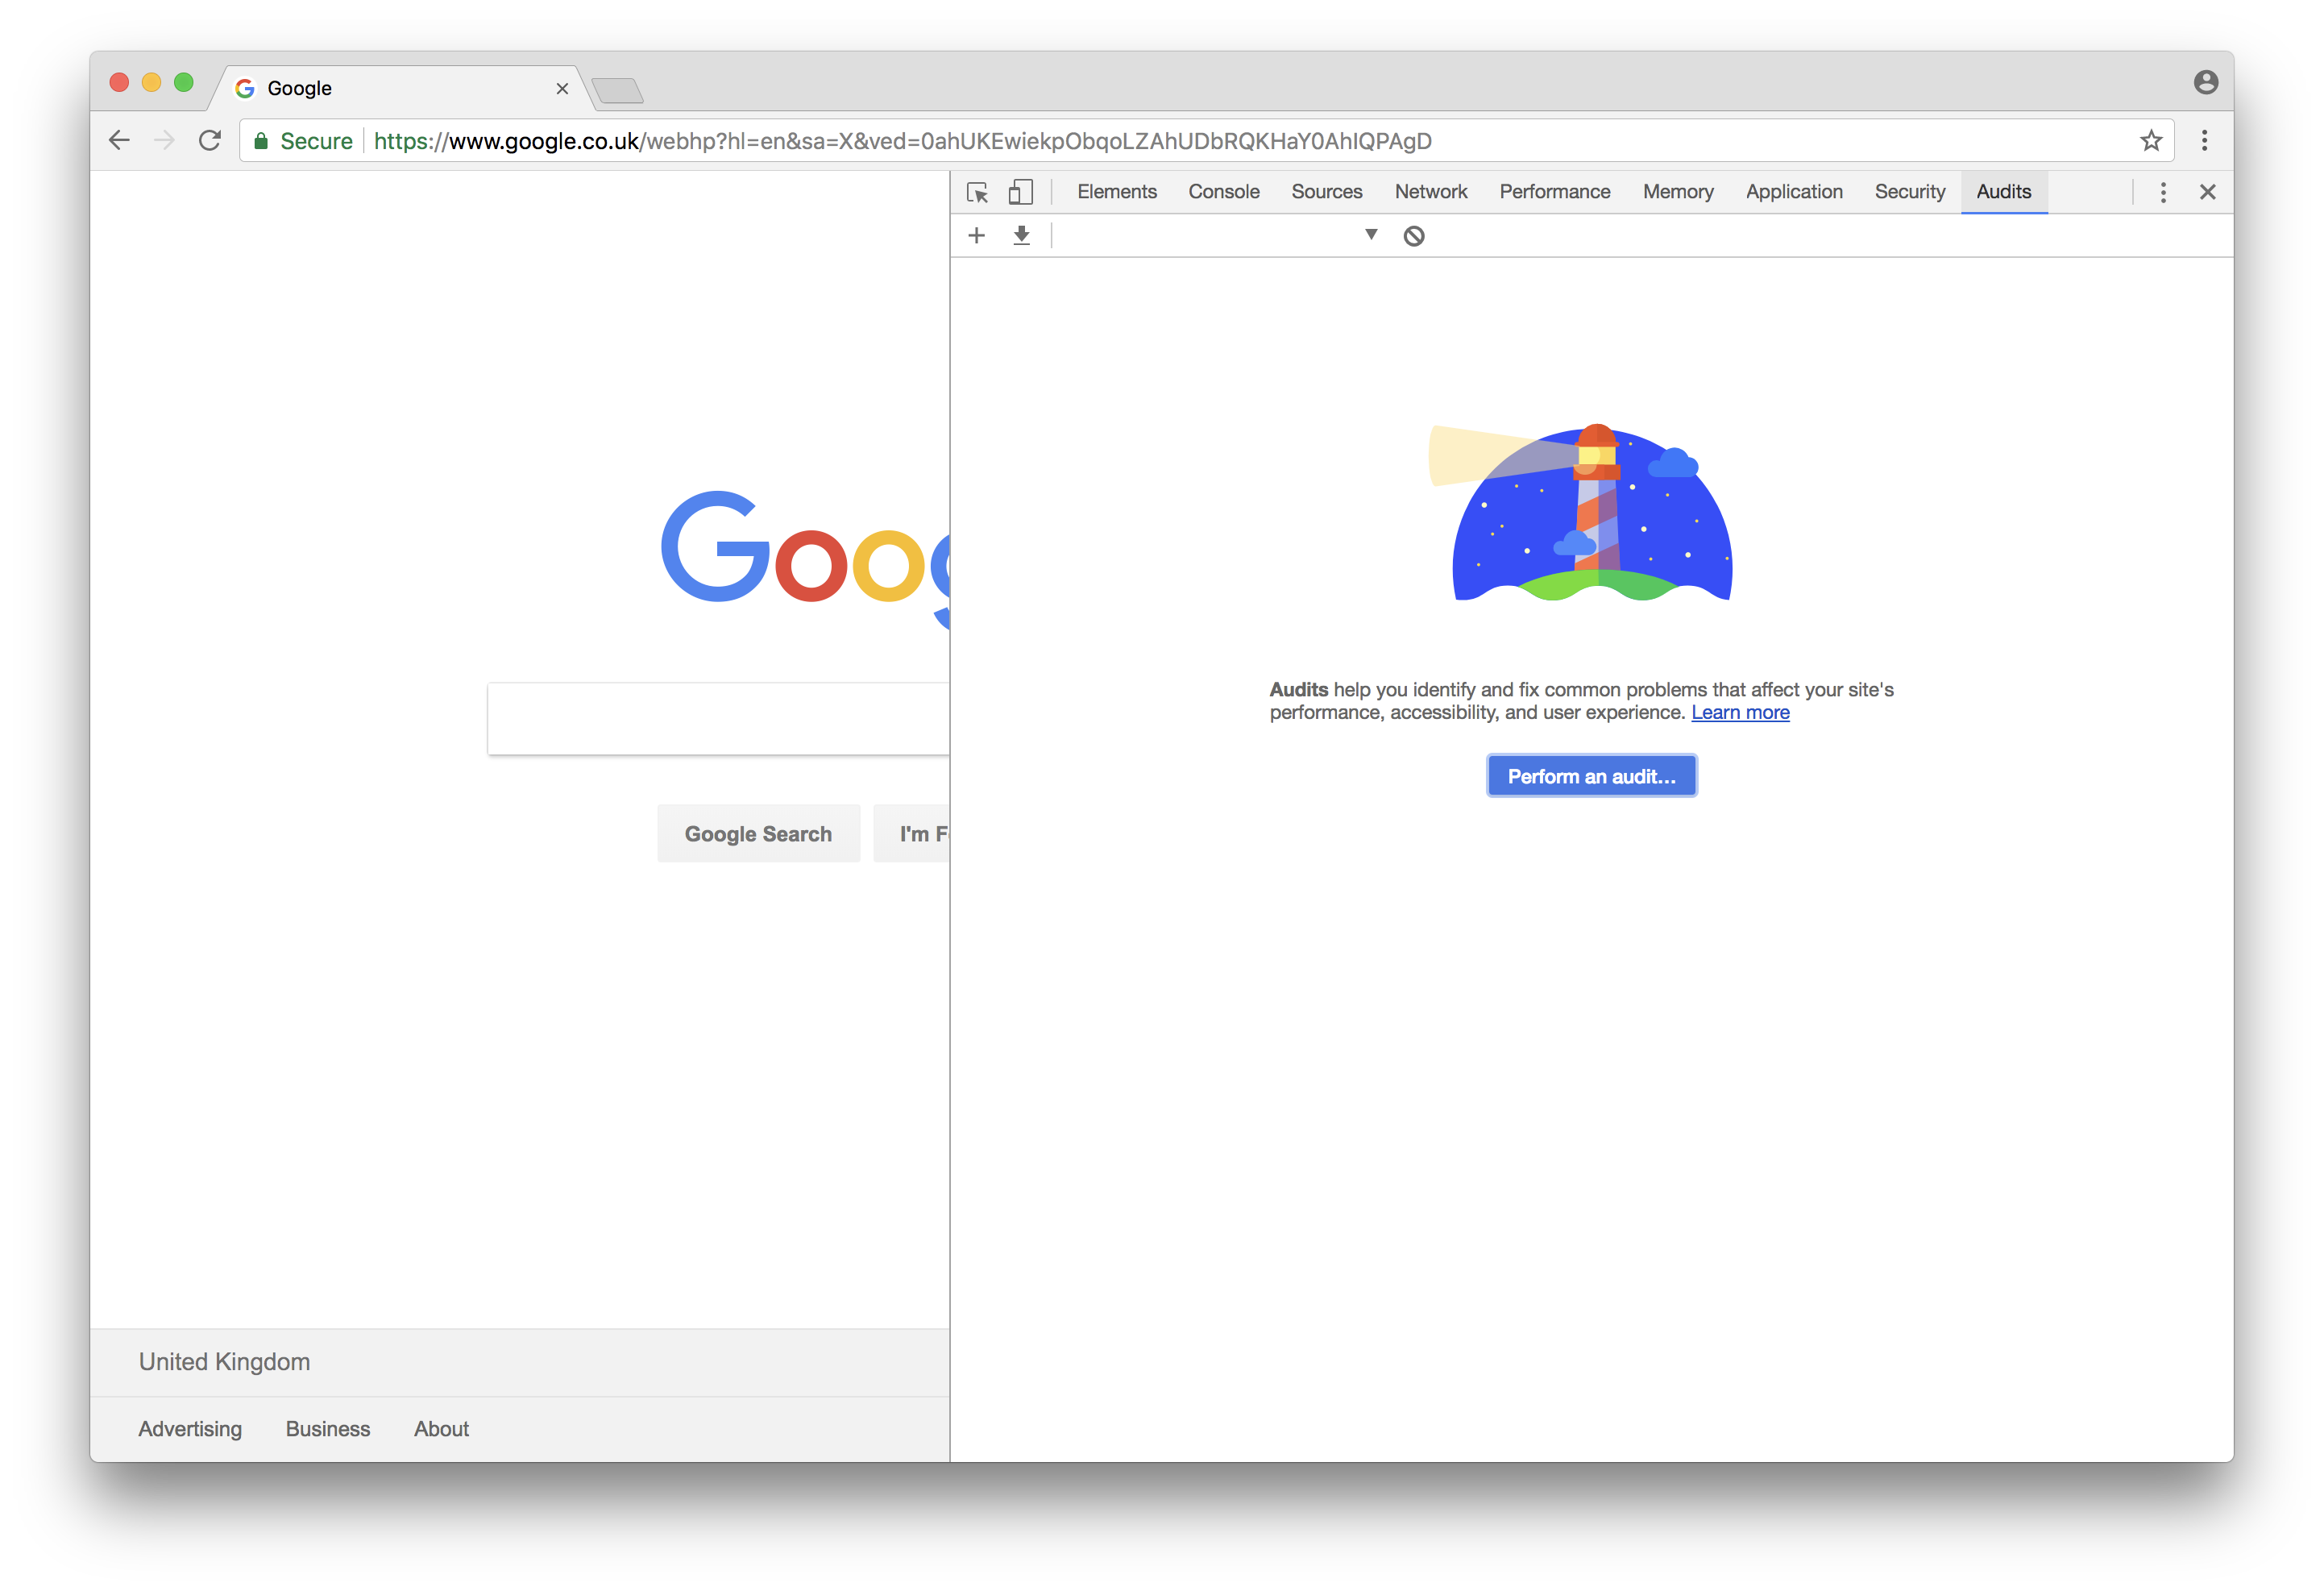
\includegraphics[width=0.8\textwidth]{figures/devtools-audits.png}
\label{fig:devtools-audits}
\end{figure}

\paragraph{} Throughout the remainder of this module, the browser tools will provide you with extrememly important insights into what your browser is doing at any given time. As your sites start to become more complex, you'll increasingly rely upon these tools to help you to track down the sources of bugs.


\section{Summary}
\paragraph{} Basically, before we can go anywhere, we should really know how we got to our current location. In this unit we've surveyed the following:

\begin{itemize}
\item A potted history of the Internet, Web, Hypertext, DOM, and Basic Web Architecture (Servers and Clients)
\item What happened technologically and socially, that lead to the situation we are in now
\item Overview of the basic things we need to know to understand how it all fits together
\end{itemize}

\paragraph{} We've also looked at the Chrome Browser features that we can exploit as a "development and learning environment" for this module.
\paragraph{} It may well be the case that you already knew about clients and servers, or HTML, CSS, and JS, or any of the other things that we've introduced in this unit. However, you should remember that this is only scratching the surface and is meant to bring us all to the same starting line, ready for the rest of the module. In all honesty, the complexity of the Web and its associated technologies, and the rapidity with which they are developing, means that there is far more to discover than it is possible for most people to know. Hopefully you've at least been introduced to some things that you hadn't thought about before. But if you are aware of all of this, then that is your cue to delve even deeper and to develop a thorough professional understanding.
\paragraph{} In summary, having read through all of the materials so far, and completed the practical work you should now have some idea of just how many different technologies interact to give us the Web that we know and love. You should also have some idea of the reasons why the Web that we have is the way that it is because of the incremental historical development of Web technologies over time, responding to user need. Finally, you should now have the minimal development environment that we'll need to progress through the rest of the units. Most important are the Chrome Browser, so that we have a default learning environment for everyone involved in the Module (which importantly incorporates useful debugging and development tools), an editor that can save plain text files (with .html, .css, and .js endings) so that we can write the source files that will make up our web pages as we progress.

%%%%%%%%%%%%%
%%%%%%%%%%%%%
%%%%%%%%%%%%%       CHAPTER 2
%%%%%%%%%%%%%
%%%%%%%%%%%%%


\chapter{Hypertext + Markup + Information + Semantics = HTML}
\label{html}
\paragraph{} 

\chapter{CSS Intro \& Overview}
\label{css}
\paragraph{} 

\chapter{HTML Page Layout Using CSS}
\label{layout}
\paragraph{} 

\chapter{Design for Hackers}
\label{design}
\paragraph{} 

\chapter{Core JS}
\label{core-js}
\paragraph{} 

\chapter{Client-Side JS: Browser APIs}
\label{browser-apis}
\paragraph{} 

\chapter{Client-Side JS: Data Storage APIs}
\label{data-storage}
\paragraph{} 

\chapter{Client-Side JS: Sound \& Vision APIs}
\label{sound-and-vision}
\paragraph{} 

\chapter{Deployment}
\label{deployment}
\paragraph{} 

%%%%%%%%%%%%%
%%%%%%%%%%%%%
%%%%%%%%%%%%%       LABS & PRACTICALS
%%%%%%%%%%%%%
%%%%%%%%%%%%%


%\part{Labs \& Practical Work}
\chapter{Learning Environment Part \#1}
\label{lab1}
\paragraph{} 


%%%%%%%%%%%%%%%%%
%%%%%%%%%%%%%%%%%
% CASE STUDIES 
%%%%%%%%%%%%%%%%%
%%%%%%%%%%%%%%%%%


%\begin{comment}
%\part{Case Studies}
%\chapter{Daybook}
%\label{daybook}
%\paragraph{}
%\end{comment}

%%%%%%%%%%%%%%%%%
%%%%%%%%%%%%%%%%%
% APPENDICES 
%%%%%%%%%%%%%%%%%
%%%%%%%%%%%%%%%%%

%\part{Appendices}

%\appendix
%\chapter{Cribsheets}
%\label{cribsheets}
%\paragraph{} These cribsheets are useful for collecting together lots of knew syntax but are no substitute for your own notes (and practise. Stuff you know is much better than stuff you can look up). Either way, as you learn new stuff you should expand these cribsheets with extra commands that you find useful.




\backmatter

\bibliographystyle{plain}

\bibliography{bib/webtech}

\end{document}


